\documentclass[11p, titlepage]{article}

\usepackage[a4paper, portrait, margin=0.9in]{geometry}
\setlength{\parskip}{1em}

\usepackage[hidelinks]{hyperref}

\usepackage{graphicx}
\graphicspath{ {./images/} }
\usepackage{caption}
\usepackage{subcaption}
\captionsetup[subfigure]{justification=centering}
\usepackage{wrapfig}
\usepackage{placeins}

\newcommand{\reconstructionleft}{0.3}
\newcommand{\reconstructionright}{0.67}

\setcounter{section}{-1}

\title{COSC470 Research Project Report\\
\bigskip
Contour Splitting for Branching Structures in \\CT Image Reconstructions}
\author{Cameron Stevenson\\[0.5cm]{\small Supervisor: Ramakrishnan Mukundan}}

\begin{document}

\maketitle
\begin{abstract}
Medical imaging modalities such as HRCT and MRI produce stacks of images depicting regions of different tissue. These image stacks can be used to reconstruct the 3D structure of internal organs. The renders or models produced are useful in diagnosis, treatment, education, surgical simulation, robot assisted surgery, and virtual reality. Correspondence methods acting on contours segmented from scan images are one such way of 3D reconstruction. These methods have difficulty in reconstructing structures such as branches and bends. There is ambiguity in contour correspondence, and extra steps must be added to point correspondence. This paper builds upon prior correspondence methods, with a new approach to point correspondence, and specifically aiming to improve on reconstructing these problematic cases. Analysis has been performed on synthetic models and real scan data. The proposed method, ``contour splitting and point angle'', handles low plane count and branching structures better than prior correspondence methods, giving more accurate reconstructions. On average the proposed method improved in reconstruction accuracy compared to the most related prior method by 15.2\%. The main contribution is the new techniques and algorithms developed for point correspondence, which may be useful in future applications.
\end{abstract}
\tableofcontents

\section{Overview}

The field of HRCT and MRI reconstructions will be introduced, followed by a broad background survey of stages in the reconstruction pipeline, with prior work relevant to this paper. The background summary will give a clear overview of what needs improvement. A method, ``contour splitting and point angle'', will be introduced which aims to satisfy these improvements. Analysis will show that this method does improve upon prior work in the intended way.

The latest version of this paper may be found here\footnote{\url{https://github.com/cstevenson3/cosc470writing/blob/main/report.pdf}}.

\pagebreak

\section{Introduction}

Medical imaging modalities such as HRCT and MRI produce stacks of images depicting regions of different tissue. These image stacks can be used to reconstruct the 3D structure of internal organs. The renders or models produced are useful in diagnosis, treatment, education, surgical simulation, robot assisted surgery, and virtual reality \cite{mackay2019robust, mukundan2016reconstruction, pan2017comparison, lobachev2021inspection}. The process of producing renders or reconstructions can be improved by reducing manual user input, improving reconstruction accuracy, or improving computational efficiency.

Prior methods include volumetric rendering (directly rendering the image data) or surface reconstruction (creating a mesh to render). Surface reconstruction methods include marching cubes, and point cloud methods such as screened Poisson. Recent papers \cite{mackay2019robust, mukundan2016reconstruction} have examined contour-based reconstructions, first segmenting images to find contours, then corresponding contours and points across slices. This paper will focus on extending this type of method.

\subsection{Motivation}

A paper by Mackay \cite{mackay2019robust} investigates the use of dynamic time warping as an algorithm for point correspondence. The analysis shows two problems impacting reconstruction accuracy. Firstly, low slice count impacts the accuracy of all reconstruction methods analysed. Secondly, branches and other such structures can be problematic to reconstruct, affecting both contour and point correspondence.

This project aims to improve the accuracy of reconstructions involving branches and other problematic structures. In particular, point correspondence will be investigated. The lungs are used as an organ of focus, as a good example structure to work on. The bronchi have many branches and the tubular shapes are easy to understand.
\pagebreak

\section{Background}

We begin with a look at typical methods in rendering or reconstructing scan data. Then, correspondence methods are looked at in depth as the approach this report builds upon.

\subsection{Overview}

Images from scans (also referred to as sections, slices, or planes) can be segmented based on intensity into pixel regions to define structure boundaries. These can be processed further by finding contours to represent these boundaries.

Volumetric rendering treats pixels in images as voxels, and a variety of rasterization and raycasting techniques are available for rendering these.

Surface rendering requires a surface be defined, either implicitly or as a mesh. Point cloud methods generate implicit surfaces, whilst meshes can be constructed via marching cubes or contour-based methods.

\subsection{Applications}

Xuyi et al. \cite{xuyi2016application} use 3D reconstructions from hip CT scans to make patient-specific surgery plans. From the model they measure the direction and degree of the acetabular fragment, and use this to guide their surgery.

Pan et al. \cite{pan2017comparison} refers to the importance of 3D reconstructions and rendering in robot-assisted surgery. With real time rendering being a priority, surface reconstructions are preferred over volume rendering. Of the four methods analysed, marching cubes was found to be the most suitable due to its speed and render quality.

Lim et al. \cite{lim2016use} found that the use of 3D printed cardiac models in education resulted in a statistically significant improvement in test scores of medical students.

Lobachev et al. \cite{lobachev2021inspection} developed a system for virtual reality rendering of reconstructions from immunohistological sections. They state that domain experts are better at analysing details in the original images, but only 3D reconstructions can offer a view of structures spanning across slices, such as blood vessels. They assert that virtual reality is the best way to allow these domain experts to view 3D reconstructions, giving them natural control over their view. High frames per second is important in VR to avoid nausea etc., and volumetric rendering may be unsuitable, with FPS as low as 25 \cite{williams2019method}. For this reason a mesh is reconstructed with marching cubes to render.

\subsection{Scanning and Image Processing}

As with most areas involving measurement of the real world, unwanted artefacts such as noise are introduced in the imaging process. There can also be variation from subject to subject and between imaging machines. Therefore standard image processing techniques are used to pick out the parts of images which are relevant to the application. Running signal processing on the 2D data (as opposed to considering the whole image stack in the reconstruction stage) reduces complexity. However techniques considering the image data from all slices have been investigated.

\subsubsection{Scanning}

The effect of slice thickness on detection has been considered by Fischback et al. \cite{fischbach2003detection}. They found that reduced slice thickness improves on small nodule detection. They compared 5mm and 1.25mm reconstruction intervals. From this we infer that higher plane count scanning through an object is better. However for small objects, say 10mm in size, we may only get up to 10 planes passing through, and so reconstruction methods need to cope with smaller plane counts.

Similarly, slice thickness has been considered for volume estimiation by Laakso et al. \cite{laakso1997mri}. They found no significant difference in estimated volume when using different slice thicknesses, although they recommend using smaller slices where possible. It is stated that smaller slice thickness results in longer scan times, so it may still be worth considering larger slice thicknesses and lower plane counts.

\subsubsection{Segmentation}

Segmentation is the process of picking out the pixels belonging to individual objects in an image. From this the projected geometry of the object onto the image can be inferred, which is then used in reconstruction or rendering. Birkfellner \cite{birkfellner2016applied} observes that organs are usually composed of multiple tissue types, which show up as different intensities under imaging. This makes segmentation ``a rather complex, specialized procedure often requiring considerable manual interaction''. We often focus on particular organs when developing segmentation methods.

Birkfellner \cite{birkfellner2016applied} covers some advanced segmentation methods. The watershed transform for example uses the physical idea of water running to the bottom of valleys in a landscape. After taking a gradient transform on an image, edges are peaks in the landscape, and the virtual water will fill up basins representing segments in the image. Various interpretations of the physical behaviour can be used.

Carr \cite{carr1996surface} refers to various morphological methods used to remove noise. An opening operation acts like a low pass filter whilst still preserving edges. Opening and closing in sequence tends to be better at maintaining the mean intensity.

Mukundan \cite{mukundan2016reconstruction} observes that in HRCT lung scans, tissue regions are ``characterized by different and easily separable intensity levels''. In this case simple thresholding can be used to pick out regions. 

\subsubsection{Contour Finding}

Rather than use pixels/voxels, some reconstruction techniques build up from contours. These contours are extracted as the boundaries of objects in each image.

Mukundan \cite{mukundan2016reconstruction} starts with a binary image after thresholding. Eroding the image with a 3x3 element then subtracting this from the thresholded image gives one pixel wide edges. Sequential edge following is used to extract contours. Discarding small contours reduces the number of contours significantly.

Pu et al. \cite{pu2008adaptive} introduce a border marching algorithm with an adaptive step size to find the outer contours of the lungs. The metric for adjusting the step size for a border segment is based on how far (at most) the segment lies from the true border. This method has the advantage of including small juxtapleural pulmonary modules in the segmentation despite their imaged intensity being dissimilar to the rest of the lung. Mackay \cite{mackay2019robust} uses this method.

\subsubsection{Contour Interpolation}

Between two slices filled with contours, new slices can be added with contours interpolated from those in the slices above and below them. Some methods are able to do this without a contour correspondence.

Barrett et al. \cite{barrett1994image} present a contour interpolation algorithm in image space based on morphological operations. An image with both contours present (as different grayscale values) is dilated until the space between contours is filled. The front where the two dilations meet is where the interpolated contour is found. It is noted that this method handles branching cases with no modification necessary.

Chai et al. \cite{chai1998contour} use partial differential equations to interpolate between contours on a terrain map. Their method produces smooth interpolations, and can handle complex shapes such as two or three branches.

\subsection{Typical Methods}

Many reconstruction methods exist. Volumetric rendering and marching cubes use the original image stack data, whilst other mesh reconstruction methods may use contours processed from scan data.

\subsubsection{Volumetric Rendering}

Each image in the image stack is treated as a slice with thickness. Thus the pixels in the image are voxels, and various volume rendering techniques can be used to directly render the data without an intermediate structural representation such as a mesh. Since every voxel may be involved in the final render, naive implementations can be expensive. Techniques to improve the render quality and performance have been investigated.

\paragraph{Rasterization}

In rasterization, the forward direction of an object's effect on an image is considered. Each voxel may directly affect the final render, or first be projected onto a intermediate object which is then itself drawn.

Splatting takes each voxel's value and ``splats'' it against the drawn image, contributing to a few pixels, with its contribution fading away from the centre pixel. Zwicker et al. \cite{zwicker2002ewa} use elliptic Gaussian kernels as the basis of the shape of each splat.

Texture-based volume rendering intersects many planes with the volume \cite{ohiotexture}. On these planes polygons are rendered, with texture mappings from their coordinates to the 3D space of the volume, to pull texture values from the voxels. The planes must not be parallel to the viewing direction.

\paragraph{Raycasting}

In raycasting, we take each pixel of the render and work backwards to find which objects affect it. Each pixel emits a ray which intersects with many voxels. The weighting of voxels is dependent on the technique.

Maximum intensity projection (MIP) is a raycasting method where rays project the most intense voxel they pass through \cite{birkfellner2016applied}. The images produced have high contrast detail and are easy to understand. Summed voxel rendering is another raycasting method where rays sum up intensities from every voxel they pass through, giving a blurred image \cite{birkfellner2016applied}.

Fishman et al. \cite{fishman2006volume} make comparisons between maximum intensity projection and other volume rendering. MIP tends to not contrast the background well with the structure of interest. Other volume rendering methods can weight voxels differently and give different tissue types different colours. 

Intersecting arbitrary rays with voxels can be computationally expensive. Shear-warp rendering solves this by using projections which make rays orthogonal to the voxel axes \cite{lacroute1994fast}. 

\subsubsection{Surface Reconstructions}

In each image of the image stack, we can see where the boundaries of tissue are. We can therefore describe the geometry of a structure as it intersects the image plane. By combining all images in the stack, a surface reconstruction of the entire object can be found, provided the relationships between slices are inferred accurately. Surfaces have the advantage of having commonplace rendering techniques, and support on 3D printers.

\paragraph{Marching Cubes}

Marching cubes \cite{lorensen1987marching} converts voxels into surfaces. Each voxel either belongs to a structure or does not, based on imaged intensity. Surface voxels (``inside'' voxels bordering ``outside'' voxels, on some isosurface) are found. Each voxel has its corners defined as inside or outside based on its neighbours, and is then assigned a set of triangles based on those corners, using a lookup table. The triangles are joined in neighbouring surface voxels to form the overall mesh. The results tend to look jagged, and smoothing is usually applied either to the mesh or during rendering for a more visually accurate output.

Newman et al. \cite{newman2006survey} have conducted a comprehensive survey of marching cubes. One problem marching cubes has is ambiguity which induces defects. The survey recommends avoiding lookup tables with reflective symmetry, where ``outside'' and ``inside'' corners of a voxel are swapped to give the same triangle set but with opposite normals. Instead only rotational symmetry (rotating corners around the voxel) is allowed. Such a lookup table was identified by Nielson et al. \cite{nielson2003marching}.

\paragraph{Point Cloud Methods}

One of the more general ways of defining a surface with incomplete data is by sampling many points from it, and making assumptions about the way these points would be connected. This is common in 3D depth scanning of exteriors of objects, where many points are sampled but the entire surface is not known and must be inferred. If we treat the boundaries of tissue regions in images as sets of points, we can apply point cloud methods to all the points gathered. The techniques can be tuned for specific applications. Approximating methods produce surfaces which lean more heavily on the assumptions made, with the points guiding the end results. This is useful when the sampling of the points is noisy. Methods which interpolate assume the points are perfect and so the surfaces produced must pass through them. It is common to define a function from 3D space to a value so that the surface should be found where the function output is zero, then an isosurface at zero is generated. A drawback of point cloud methods is that the explicit relations between points on the same contour are lost. In addition, when planes are more separated, artefacts tend to appear.

\subparagraph{Models}

Braude et al. \cite{braude2007contour} employ Multi-level Partition of Unity (MPU) implicit models to generate isosurfaces from. MPU closely approximates Euclidean distance near points. This method requires surface normals. 

Guennebaud et al. \cite{guennebaud2007algebraic} fit algebraic spheres to point sets to construct surfaces. Their method (APSS) performs better than prior methods on sharp features and sparse data.

Oztireli et al. \cite{oztireli2009feature} combine Moving Least Squares (MLS) with local kernel regression to obtain Robust Implicit Moving Least Squares (RIMLS). This method reconstructs sharp (non-smooth) corners more accurately than APSS.

Taubin et al. \cite{taubin2012smooth} demonstrate colour maps extrapolated from source points onto a reconstructed surface.

\subparagraph{Estimating Normals}

Some of the methods above require normals for each point. Estimating normals from the points sampled requires some understanding of the structure itself.

Mitra et al. \cite{mitra2003estimating} use least squares distance to fit a plane to a neighbourhood of points for each point in the cloud. There is a sweet spot for the radius of the neighbourhood used. Small radius makes noisy points have more impact on the plane found, and large radius allows for surface curvature to introduce error. 

\paragraph{Mesh Rendering}

Mackay \cite{mackay2019robust} states that surface rendering is not as widely implemented as volume rendering in medical contexts. However mesh rendering is abundant in literature from applications such as video games. Should mesh reconstruction become more accurate and faster, more implementations of mesh rendering for medical imaging may become available.

\subsection{Testing}

The end aim of these reconstructions and renders is to give humans a better visualisation of internal structures. However to compare methods objective testing is required. Requiring human experts to come to a consensus on desired outputs is resource consuming for stages such as image segmentation, and infeasible for complex structures such as meshes. Therefore metrics and repeatable methods have been devised to test algorithms.

\subsubsection{Measuring Similarity in Segmentation}

Pixel-wise XOR operations are common, simply working out where an ideal segmentation and an output segmentation differ.

Pu et al. \cite{pu2008adaptive} use a reference segmentation contour (defined by experts), and evaluate the distribution of distance error along their result contour from this reference. 

\subsubsection{Generating Models}

It is difficult to obtain real models of internal structures. Techniques to generate synthetic models suitable for testing have been developed.

Mackay \cite{mackay2019robust} uses Blender3D to create test models, by creating surface of revolutions about bezier curves. Multiple surfaces are merged for more complex structures such as branches. The main intent here was to create simple models of problem structures. Contours can be sampled from these models by plane intersections.

Mackay \cite{mackay2019robust} also proposes an alternative method of generating test data, where a side view of a branching structure is drawn in black. An inter-slice distance is defined to separate rows. Each row is scanned for black pixels. When a black pixel is encountered, a contour is generated by revolving points about this pixel location. Noise can be added in. Where contours intersect, they are merged. This allows for branching structures to be generated by this method.

Pluta et al. \cite{pluta2012new} propose a rule-based method of generating lung models, including deformations and noise. Their rules are based on airflow and measured constants, and the distribution of final bronchioles in a lung. Their results are suitably accurate for testing all parts of lung reconstruction methods.

\subsubsection{Measuring Similarity in 3D Models}

Mackay \cite{mackay2019robust} uses Hausdorff distance (essentially a maximum deviation between point sets) to measure mesh similarity. Points are sampled from a ground truth model and the nearest distance is found to the reconstructed model.

Meshes can be sliced at the same heights and compared slicewise to reduce similarity to a 2D problem.

Shum et al. \cite{shum19963d} compare simple 3D objects by comparing the curvature of points based on spherical coordinates. This could be applied locally on more complex medical reconstructions.

\subsection{Performance}

Recent papers in medical imaging reconstructions tend to have an emphasis on taking advantage of modern hardware. This can be achieved through parallelization or GPU implementations.

Saxena et al. \cite{saxena2013image} describe parallel techniques for various image processing tasks such as segmentation and noise reduction. The main idea is to tile an image and let different processors work on different tiles, then deal with the borders when recombining the tiles. They found their parallel implementation to be 2.5 times faster than a sequential implementation.

Alsmirat et al. \cite{alsmirat2017accelerating} investigate pure GPU and hybrid CPU-GPU implementations of segmentation of medical images. They found that both outperform a CPU only implementation, and the hybrid method performs the best.

\subsection{Correspondence Methods}

Contour-based mesh reconstruction first gathers contours from image data, then corresponds contours between slices. Matched contours then go through point correspondence and triangulation to produce a final mesh. This approach to mesh reconstructions is the focus of this paper.

\subsubsection{Contour Correspondence}

\begin{wrapfigure}{r}{0.6\textwidth}
\centering
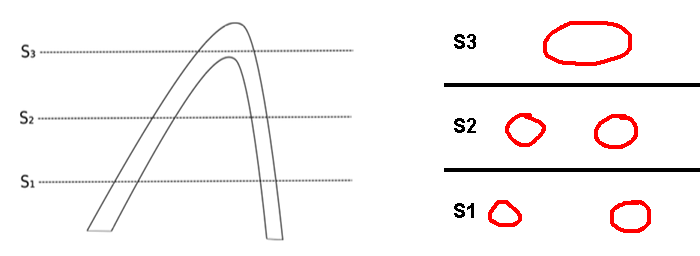
\includegraphics[width=0.58\textwidth]{diagrams/contours_sampled}
\caption{Example of scanned structure and contours extracted \label{fig:contours_sampled}}
\end{wrapfigure}

Rather than lose the relationship between points, the original contours can be used in creating a surface reconstruction. Working out which contours on which slices represent a connected tissue in the original structure is called contour correspondence, and the resulting correspondences are used in later steps of reconstruction.
\newline
\linebreak
Herbert et al. \cite{herbert2001contour} classify correspondence algorithms into four types. \begin{itemize}
\item Manual methods use user input to connect contours. This is time consuming for large datasets.
\item Local algorithms takes pairs of slices at a time and considers contour matchings between these.
\item Global algorithms look for contour pairings across all sections.
\item Growing algorithms create a hierarchy of components, attempting to join unmatched contours onto existing components if suitable.
\end{itemize}

Contour centroid position comparison is common in local algorithms.

Herbert et al. \cite{herbert2001contour} suggest growing objects one contour at a time instead of considering pairings of contours globally. In preprocessing spacial information is gathered such as contour characteristics (position, shape, size), intra-sectional relationships between contours (to validate complex structures later), and inter-sectional relationships. Contour relationship metrics include distance between centroids, distance between major/minor axes, minimum bounding rectangle overlap, shape comparison via compactness ratios, and surroundness (how deep the contour is nested in larger contours).

Herbert et al. \cite{herbert2001contour} include semantic information given by the user on the expected components in a reconstruction, and their spatial relation to each other. A starting contour is found for each component before the growing process starts.

Mukundan \cite{mukundan2016reconstruction} begins point correspondence without an explicit contour correspondence already found. If two point correspondences are found as neighbours belonging to the same pair of contours, the search for further point correspondences is narrowed to these two contours. This effectively gives a temporary contour correspondence.

\subsubsection{Point Correspondence}
Point correspondence is an optional step in surface reconstructions, where points on matched contours are matched to each other as a precursor to triangulation.

Mukundan \cite{mukundan2016reconstruction} uses distance in the XZ plane as a metric for matching points. Other optional constraints include matching the next point close to the previous point.

\begin{figure}[h]
     \centering
     \begin{subfigure}[b]{0.2\textwidth}
         \centering
         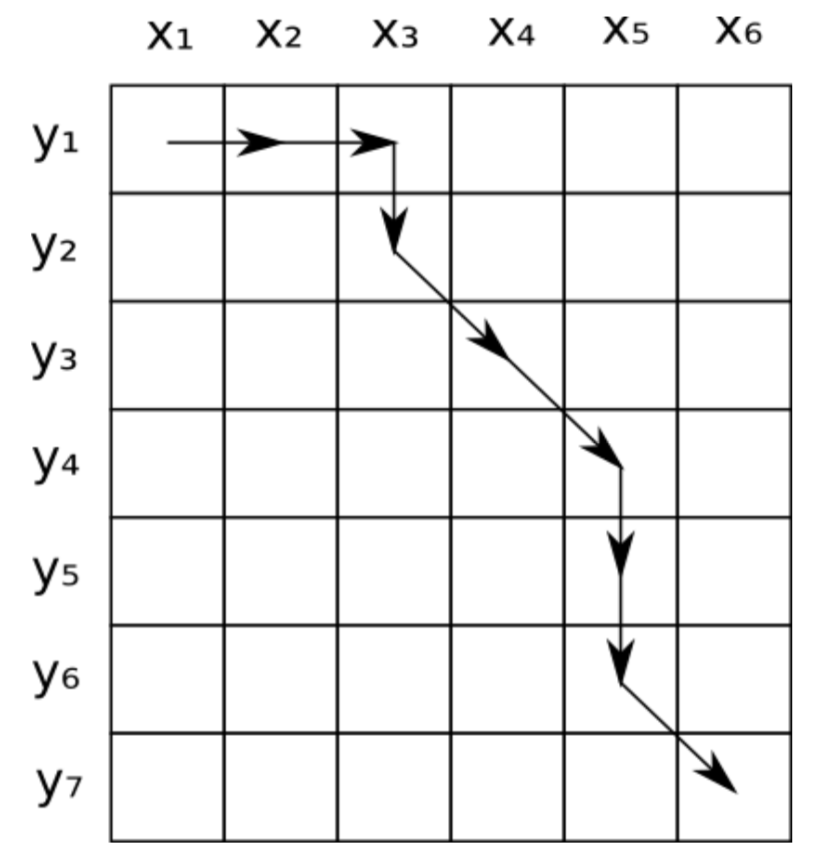
\includegraphics[width=\textwidth]{diagrams/dtw1}
         \caption{DTW path through cost matrix}
         \label{fig:dtw1}
     \end{subfigure}
     \hfill
     \begin{subfigure}[b]{0.6\textwidth}
         \centering
         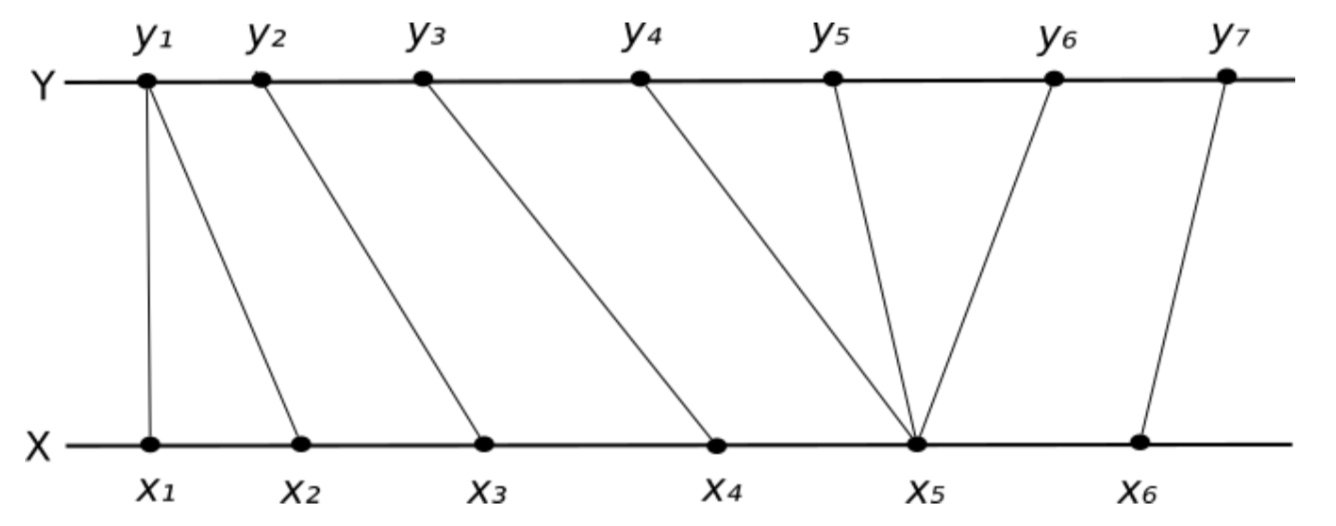
\includegraphics[width=\textwidth]{diagrams/dtw2}
         \caption{Point correspondence}
         \label{fig:dtw2}
     \end{subfigure}
        \caption{DTW path finding through a cost matrix to give a point correspondence \cite{mackay2019robust}}
        \label{fig:dtw}
\end{figure}

Mackay \cite{mackay2019robust} proposes Dynamic Time Warping (DTW) as a method of point correspondence. DTW is intended to match features on the same structure across different times. In point correspondence, it matches points on contours which are from the same structure but in different slices, so slightly warped. At any time during DTW a pair of points from both contours is matched, then the next points in both contours are considered as matches for the current points. A cost matrix is populated based on point distance, then a path is found aiming to minimise global distance (See Figure \ref{fig:dtw}). DTW has some basic constraints when finding a warp path, but Mackay suggests adding further constraints as a potential improvement. It tends to be that as planes are more separated, the contours undergoing point correspondence are more dissimilar, and DTW performs worse in reconstructing these.

\subsubsection{Mesh Triangulation}

A surface can be represented as a set of primitive elements, with triangles being the simplest. They are defined by three points in 3D space. The final step of mesh reconstruction is taking the relationships inferred by contour and point correspondence, and generating triangles to connect points whilst taking these relationships into account.

Mackay \cite{mackay2019robust} begins with two ordered sets of points X and Y, from the two contours matched, with some edges provided by point correspondence. As a result of the constraints on DTW, there are three cases for each point $x_{m}$ on the first contour:
\begin{itemize}
\item $x_{m}$ has an edge with $y_{n}$ and $x_{m+1}$ has an edge with $y_{n+1}$. These points are direct neighbours on their respective contours, and form a quad which is trivial to triangulate.
\item $x_{m}$ has edges with a sequence of points $\{y_{n}, y_{n+1}, ..., y_{n+i}\}$. $x_{m}$ has a one-to-many point correspondence with these points. This can be triangulated with a triangle fan centering about $x_{m}$.
\item Each point in the sequence $\{x_{m}, x_{m+1}, ..., x_{m+i}\}$ has edges with a point $y_{n}$. This is the opposite of the previous case and can likewise be triangulated with a triangle fan centering about $y_{n}$.
\end{itemize}
Li et al. \cite{li2021method} observe that when m and n differ greatly, one-to-many point correspondences are common, and the triangulation becomes rough.

\subsubsection{Branching Problem}

A simple structure is easy to infer from its images. On every slice the structure is present in, we see one contour, and all these contours are similarly positioned and shaped in adjacent slices. More complex structures such as a branch show up differently, and it becomes harder to infer the original structure. Contour correspondence must be adjusted to deduce these unusual structures when they appear. Even when the general layout of the original structure is inferred through contour correspondence, point correspondence and mesh triangulation can be difficult when the shapes of contours change suddenly.

Mackay \cite{mackay2019robust} looks for lung branches as one contour approximately splitting in half into two contours, for contour correspondence.

\begin{figure}[h]
     \centering
     \begin{subfigure}[b]{0.3\textwidth}
         \centering
         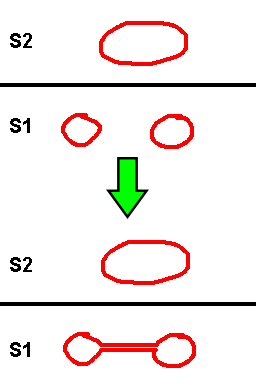
\includegraphics[width=\textwidth]{diagrams/contour_merging}
         \caption{Contour merging for branching cases}
         \label{fig:contour_merging}
     \end{subfigure}
     \hfill
     \begin{subfigure}[b]{0.4\textwidth}
         \centering
         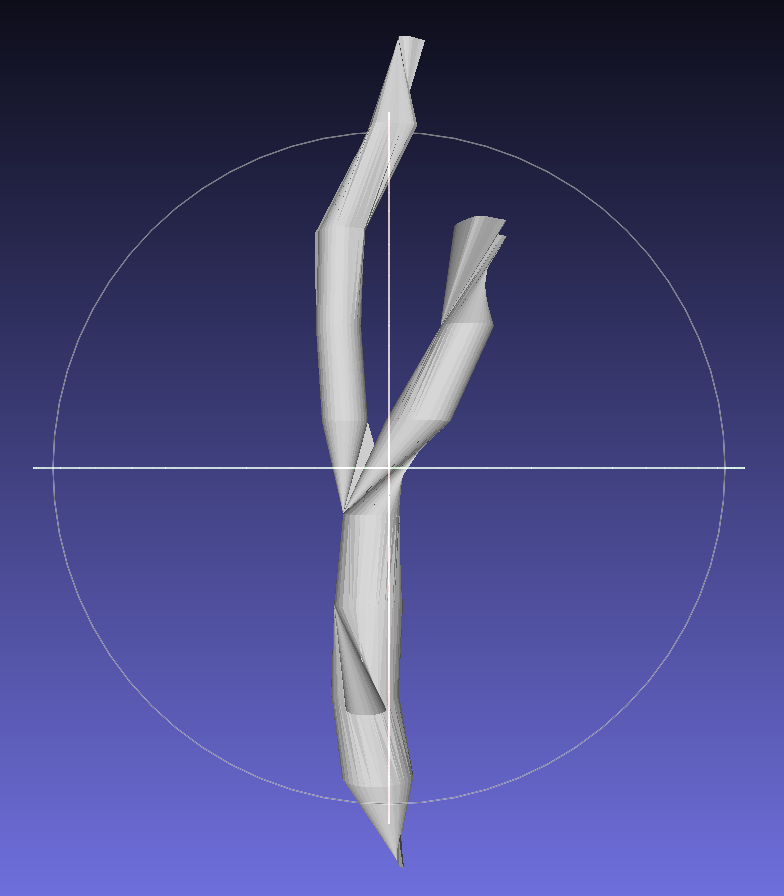
\includegraphics[width=\textwidth]{reconstructions/dtw-multi-branch-10}
         \caption{DTW pathing issues on branching cases}
         \label{fig:dtw_issues}
     \end{subfigure}
        \caption{Mackay contour merging and DTW}
        \label{fig:dtw}
\end{figure}

Mackay \cite{mackay2019robust} uses contour merging to help DTW point correspondence in the branching case. In a contour correspondence where there is a slice with a single contour and a slice with two contours, the two contours on the same slice are merged at their nearest point to give one larger contour (See Figure \ref{fig:contour_merging}). Point correspondence between the single contour and the merged contour can then proceed as normal. In some branching cases however, the triangulated mesh is twisted, as though DTW has not matched the correct points together (See Figure \ref{fig:dtw_issues}). This problem is left for further research.

\subsection{Background Summary}

Scans have multiple planes separated by some distance. For the same spatial resolution, smaller objects will have fewer planes scanning through them. Alternatively, for a given sized object, lower plane counts are better for lowering scan time. Reconstruction methods which can handle lower plane counts should give more accurate reconstructions of smaller objects, or allow for shorter scan times.

General methods related to volumetric rendering and mesh reconstructions have been applied to scans. These all have some drawback. For volumetric rendering it is the render time, for marching cubes it is the jagged meshes, and for point cloud methods it is the approximation of structure.

Counter-based correspondence methods aim to solve these issues. Contour correspondence and point correspondence are achieved through variations of Euclidean distance and other metrics. Mackay was able to achieve similar or better accuracy to prior methods with substantially lower triangle count. Mackay found that branches and other structures cause problems in both contour and point correspondence. His method using DTW, like others, becomes less accurate as plane count decreases.

A new point correspondence method can improve upon prior approaches by reconstructing branches and other structures more accurately, and handling lower plane counts better.
\pagebreak

\section{Method}

In this section I detail how a new point correspondence method has been constructed, with the intention of handling branching structures and lower plane counts better.

\subsection{Proposal}

The proposed system consists of:
\begin{itemize}
\item Contour Splitting, a new approach to enabling point correspondence on branches and other structures
\item Point Angle, an alternative algorithm for point correspondence.
\end{itemize}

\subsubsection{Contour Splitting}

For brevity, contour correspondences of 1-to-2 will be considered. Point correspondence algorithms act on 1-to-1 contour matchings, so 1-to-2 cases must be reduced to these. 

Mackay's approach was contour merging, where the 2 contour side of the correspondence is merged. The closest pair of points across the contours is found, to join them into a single contour (See Figure \ref{fig:contour_merging}). This gives a single 1-to-1 case for point correspondence to act on. A disadvantage of this method is that the merged contour has an unusual shape, which can cause point correspondence algorithms to behave poorly.

\begin{figure}[h!]
\centering
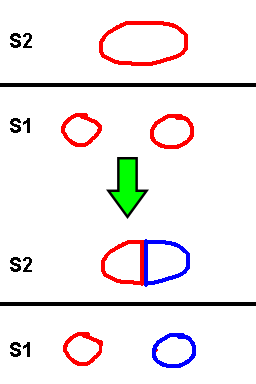
\includegraphics[width=0.28\textwidth]{diagrams/contour_splitting}
\caption{Contour splitting \label{fig:contour_splitting}}
\end{figure}

The proposed technique instead splits the 1 contour side of the correspondence. The best fit line to divide the 2 contour side is found, giving the angle of the line to split the 1 contour (See Figure \ref{fig:contour_splitting}). Each half of the split 1 contour is paired with its corresponding contour on the 2 contour side. This gives two 1-to-1 cases for point correspondence to act on. The contours produced are well shaped and suitable for point correspondence algorithms designed for simpler cases.

\begin{figure}[h!]
     \centering
     \begin{subfigure}[b]{0.35\textwidth}
         \centering
         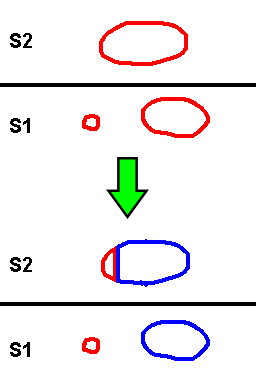
\includegraphics[width=\textwidth]{diagrams/ratio_of_area}
         \caption{Ratio of areas under splitting}
         \label{fig:ratio_of_area}
     \end{subfigure}
     \hfill
     \begin{subfigure}[b]{0.35\textwidth}
         \centering
         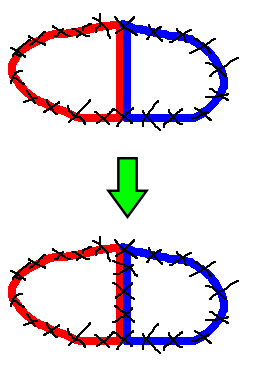
\includegraphics[width=\textwidth]{diagrams/split_line_points}
         \caption{Additional points added to split line}
         \label{fig:split_line_points}
     \end{subfigure}
        \caption{Implementation features for contour splitting}
        \label{fig:contour_splitting_features}
\end{figure}

Adjustments can be made to the position of the split line to improve accuracy. 
\begin{itemize}
\item The ratio of contour areas on the 2 contour side can be reflected in the split contour by adjusting which points the split line connects to (See Figure \ref{fig:ratio_of_area}). This preserves the internal cross section of each branch half as they join. 
\item To achieve a smooth point correspondence along the inside of the branch (where the branches join each other), the split line must have points added along it (See Figure \ref{fig:split_line_points}). This is in proportion to the number of points on the original contour.
\item The split line may also be adjusted in height, to reflect the likelihood the branch split is somewhere between the two planes of contours. With no further calculation, the height is assumed to be halfway. A semi-circular curve (changing in height above the split line) creates a split line joint which mimics the intersection of two cylinders, which is approximately what is expected from two branches coming together.
\end{itemize}

\subsubsection{Point Angle}

\begin{wrapfigure}{r}{0.3\textwidth}
\centering
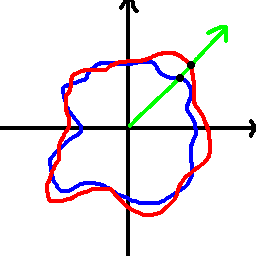
\includegraphics[width=0.28\textwidth]{diagrams/point_angle}
\caption{Correspondence by point angle \label{fig:point_angle}}
\end{wrapfigure}

Prior methods of point correspondence consider the Euclidean distance between points on corresponded contours. The proposed algorithm instead considers similar angular distance relative to the contour's centroid (See Figure \ref{fig:point_angle}). For contours where every border point can be seen from the centroid (similar to star-shaped polygons), the angular distance metric is monotonically increasing as we progress along the contour's specified order (if we start from the smallest angle point). In point correspondence, the contours' point angle metrics are leapfrogged between to join points (See Figure \ref{fig:point_angle_leapfrogging}). This leapfrogging assumes the monotonically increasing property. For contours which ``double back'' (are not star-shaped), the monotonically increasing property can be enforced when filling in the point angle metric, by recording the previous angle if the current angle is smaller.

\begin{wrapfigure}{r}{0.3\textwidth}
\centering
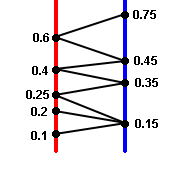
\includegraphics[width=0.28\textwidth]{diagrams/point_angle_leapfrogging}
\caption{Leapfrogging of point angle metric \label{fig:point_angle_leapfrogging}}
\end{wrapfigure}

This can lead to sections of points with the same point angle metric, and leapfrogging which produces unideal many-to-one mappings. To counter this, a second metric is added, which is simply progression along the number of points in the contour (normalized), starting from the same point as the angle metric. The angle and progression metrics are weighted and summed before the leapfrogging correspondence. This progression metric is actually well suited to contour data with similarly distanced points, which is what we get from uncompressed image contours. In these cases it may be suitable to only use progression.

\subsection{Implementation}

Mackay's report provides a complete implementation of contour and point correspondence\footnote{\url{https://drive.google.com/open?id=1EHIx3dOOwcP1KTxWxhv8NWyROHAyVZ-P}}. Contour correspondence is implemented by checking the distance between centroids relative to the radius of the contours, which indicates if there is any overlap. The complete implementation was modified to add the options of contour splitting and point angle for point correspondence. The modified source code and tools are available here \footnote{\url{https://github.com/cstevenson3/cosc470code}}.

This paper contributes a new tool for testing. A python script has been developed to automate reconstruction and analysis of multiple models and plane counts. The script calls the reconstruction binary and feeds it every combination of model and plane count to obtain reconstructions. PyMeshLab \cite{pymeshlab} is then used to call the Hausdorff distance filter with reconstructions and their original counterparts, giving measurements which are then stored in a JSON file. The script includes methods to filter this file, to quickly look up measurements across different reconstruction methods for a given model and plane count.
\pagebreak

\section{Analysis}

To analyse the effectiveness of the proposed method in improving reconstruction accuracy, synthetic models are intersected with planes to give contours of points, which are then given as input to reconstruction. These reconstructions from different methods are compared to the original and against each other. The observations are then confirmed with objective measurements such as Hausdorff distance. Finally a reconstruction from real lung scans will be explored.

Mackay compared his method to typical non contour-based methods, the results of which are available in his paper \cite{mackay2019robust}. For simplicity we will only compare the proposed method to his method.

\subsection{Ground Truth}

For ground truth I used the same synthetic models Mackay generated for analysis (See Figure \ref{fig:original_models}). These can be downloaded standalone\footnote{\url{https://drive.google.com/open?id=1QYsQa-qsz9mwDRz_nk4ohtD4pITV9AD3}}, but are also included alongside my implementation\footnote{\url{https://github.com/cstevenson3/cosc470code}}. Planes are intersected with the models to give the contours of points expected from scanning and segmenting a real object of the same shape. Plane counts of 10, 20, 30, 40 and 50 are used to emulate different scan slice thicknesses.

Additionally, Meshlab was used to copy specific sections of these models into new files, to focus reconstructions on the difficult cases the proposed method is intended to improve on. These are named after the original model and which slice range (based on the 10 slice levels version) is being copied.

\begin{figure}[h!]
     \centering
     \begin{subfigure}[b]{0.3\textwidth}
         \centering
         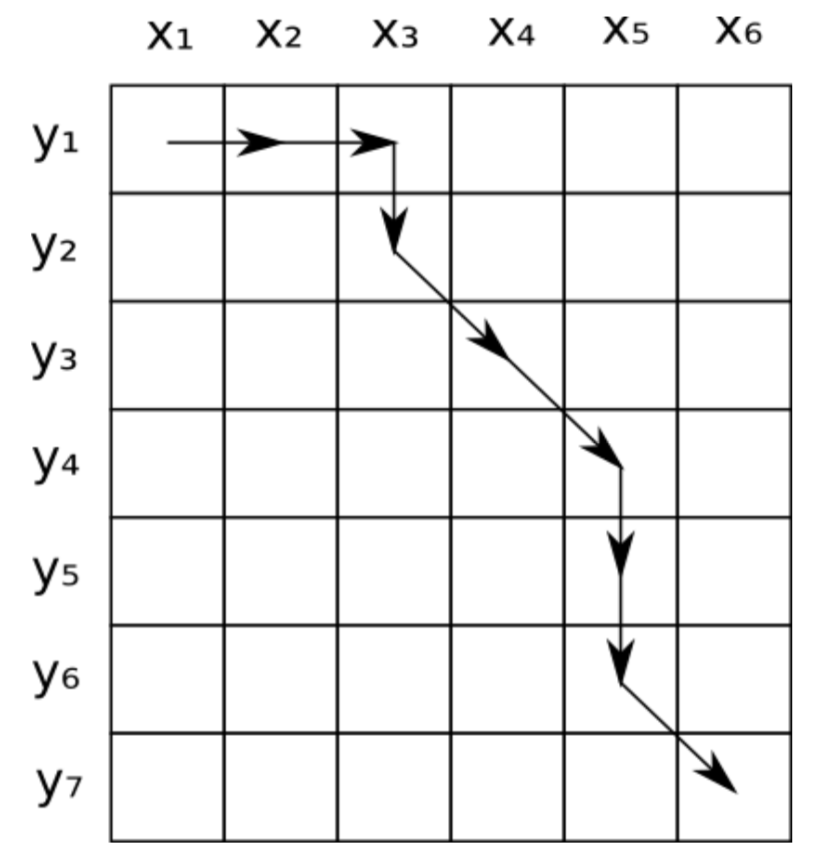
\includegraphics[width=\textwidth]{originals/simple}
         \caption{simple}
         \label{fig:simple}
     \end{subfigure}
     \hfill
     \begin{subfigure}[b]{0.3\textwidth}
         \centering
         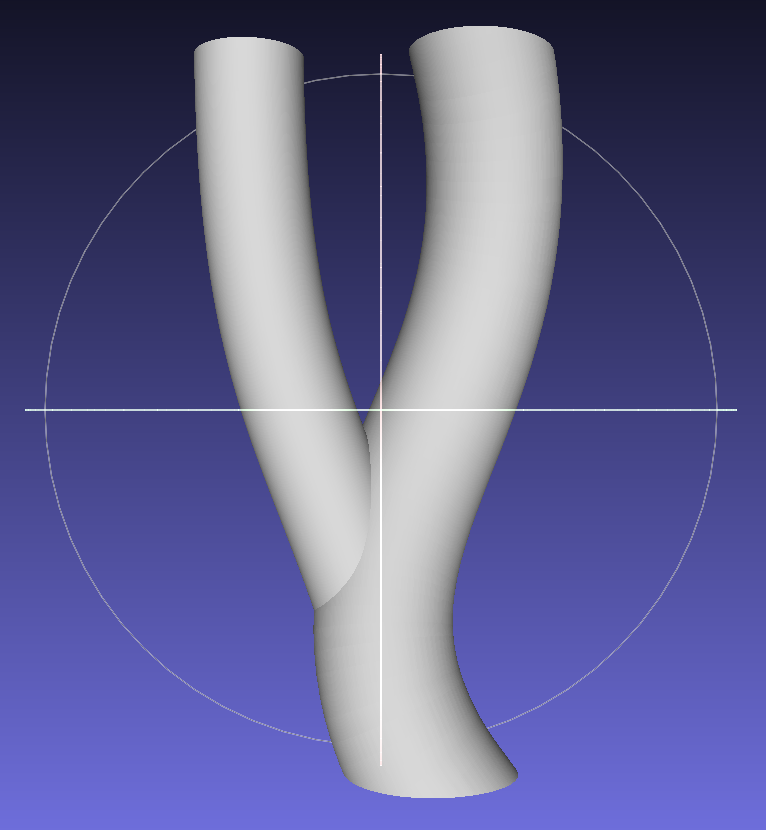
\includegraphics[width=\textwidth]{originals/simple-branch}
         \caption{simple-branch}
         \label{fig:simple_branch}
     \end{subfigure}
     \hfill
     \begin{subfigure}[b]{0.3\textwidth}
         \centering
         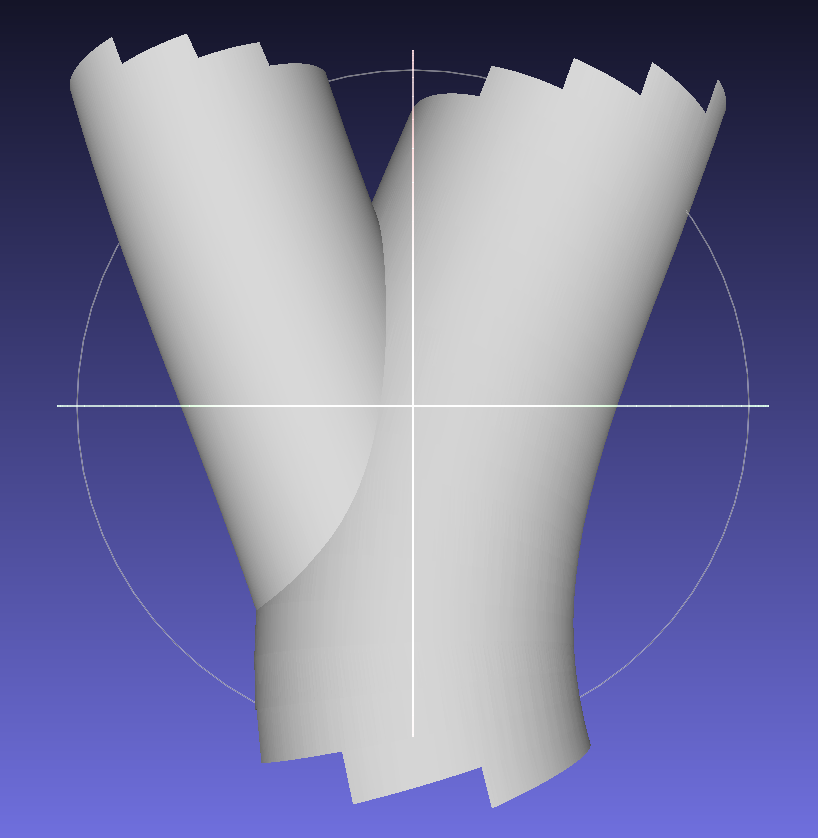
\includegraphics[width=\textwidth]{originals/simple-branch-2-6}
         \caption{simple-branch-2-6}
         \label{fig:simple_branch_focussed}
     \end{subfigure}
     \hfill
     \begin{subfigure}[b]{0.3\textwidth}
         \centering
         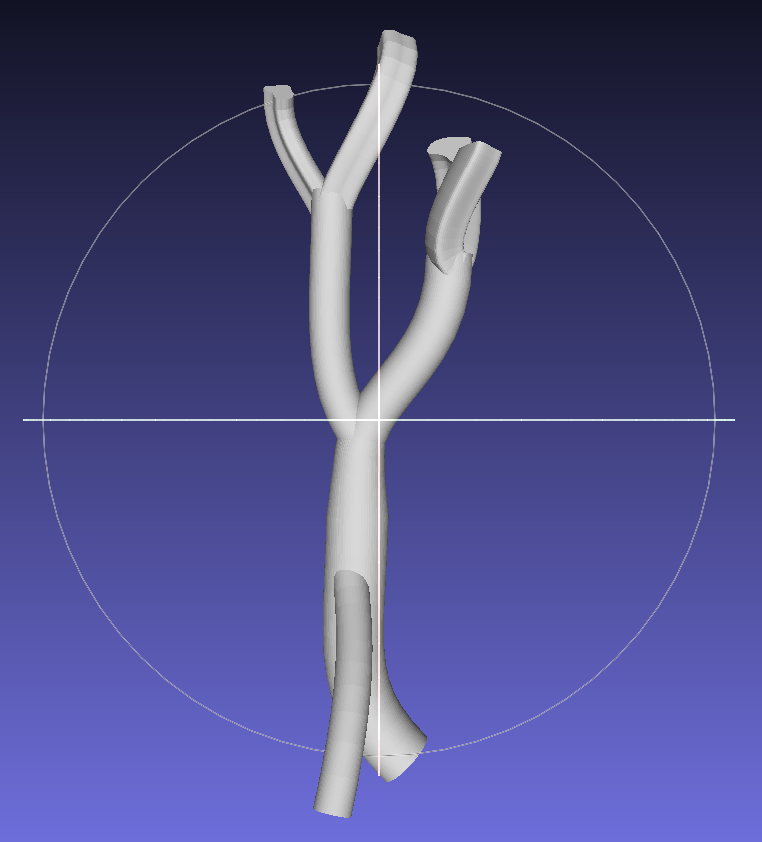
\includegraphics[width=\textwidth]{originals/multi-branch}
         \caption{multi-branch}
         \label{fig:multi_branch}
     \end{subfigure}
     \hfill
     \begin{subfigure}[b]{0.3\textwidth}
         \centering
         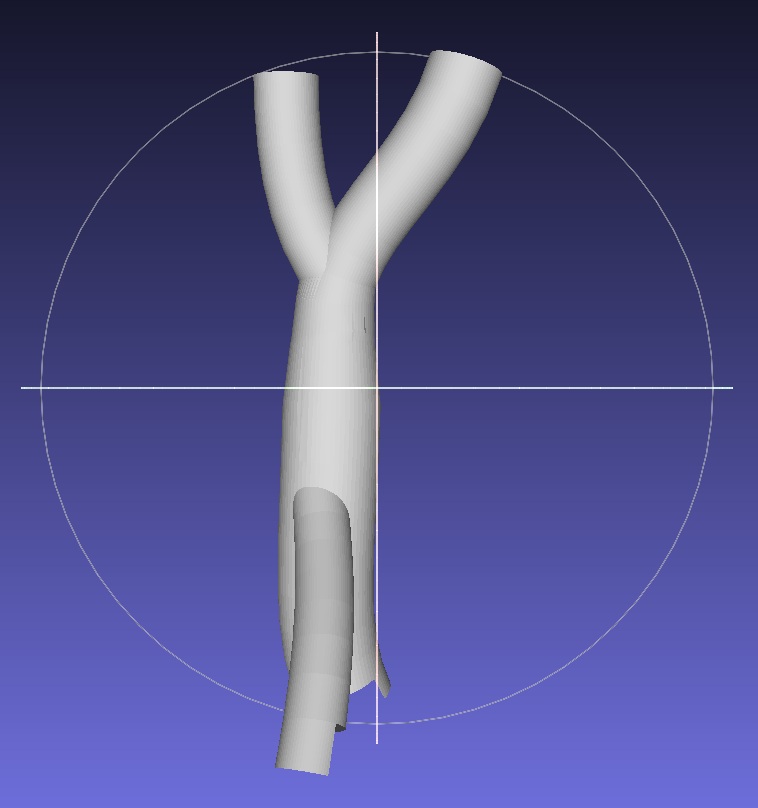
\includegraphics[width=\textwidth]{originals/multi-branch-2-7}
         \caption{multi-branch-2-7}
         \label{fig:multi_branch_focussed}
     \end{subfigure}
     \hfill
     \begin{subfigure}[b]{0.3\textwidth}
         \centering
         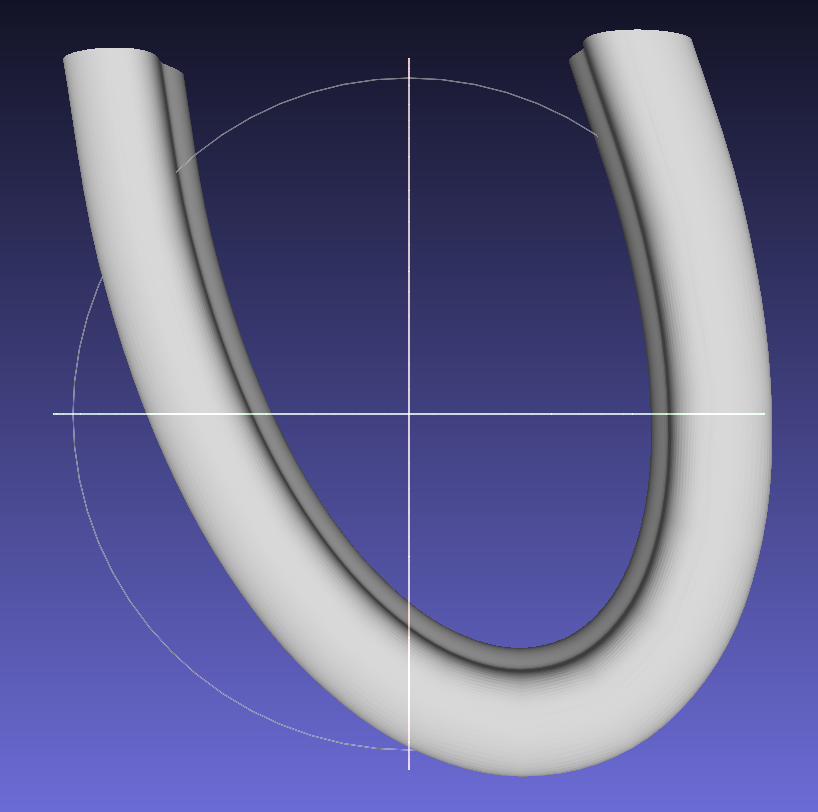
\includegraphics[width=\textwidth]{originals/bend}
         \caption{bend}
         \label{fig:bend}
     \end{subfigure}
        \caption{Original Models}
        \label{fig:original_models}
\end{figure}

\subsection{Measurements}

For reconstruction accuracy, Mackay used the Hausdorff distance filter built into Meshlab, which takes as input a sampled mesh (the mesh to sample points from), and a target mesh (to find the closest distance from each sample point). Many points are sampled and mean distance is reported. Lower mean distance is better. I may refer to the forward direction as when the original synthetic mesh is the sampled mesh, and the reconstructed mesh is the targest mesh, with reverse being the opposite. 

The filter also has parameters related to sampling, such as whether vertices, edges, or faces are sampled. The choices of sample/target meshes and these parameters are important, as the nature of how the models and reconstructions are generated affect different methods differently. For example, all vertices in Mackay's reconstructions are the original points given by plane sampling, and so lie on a face in the original mesh. Hence the reverse Hausdorff distance filter with only vertices sampled gives a measurement of zero. Whereas the proposed method adds additional points, and so is unlikely to achieve this zero measurement. For this reason only faces will be sampled. When it comes to direction, extraneous faces on a target mesh may reduce Hausdorff distance, but extraneous faces on a sampled mesh increase Hausdorff distance (usually the preferred interpretation). For this reason, in same examined cases a direction may be omitted, for reasons which will be explained.

For contour merging and DTW, Mackay's implementation is used. For the proposed method, the same implementation is used except where contour splitting and point angle replace the point correspondence stage. To start with, 50\% angle weight (and 50\% progression) is used in the point angle metric.
\pagebreak

\subsubsection{Simple Model Reconstruction}

A simple tube is reconstructed.

\begin{figure}[h!]
     \centering
     \begin{minipage}[b]{\reconstructionleft\linewidth}
       \subcaptionbox{Original}
       {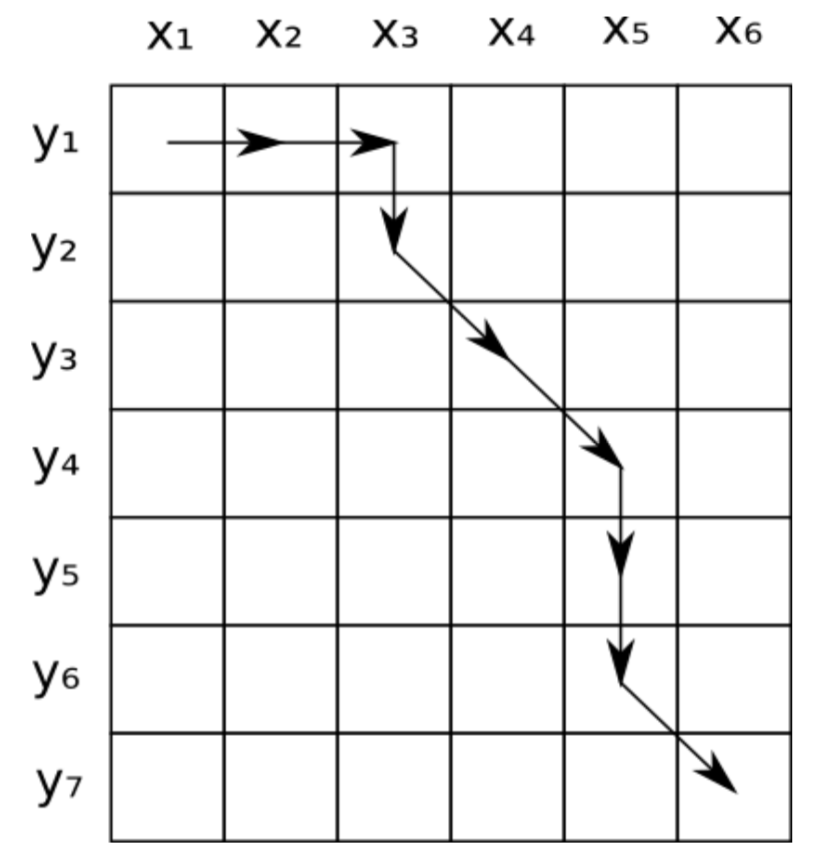
\includegraphics[width=\linewidth]{originals/simple}}%
     \end{minipage}%
     \hfill
     \begin{minipage}[b]{\reconstructionright\linewidth}
       \subcaptionbox{DTW 50 planes}
       {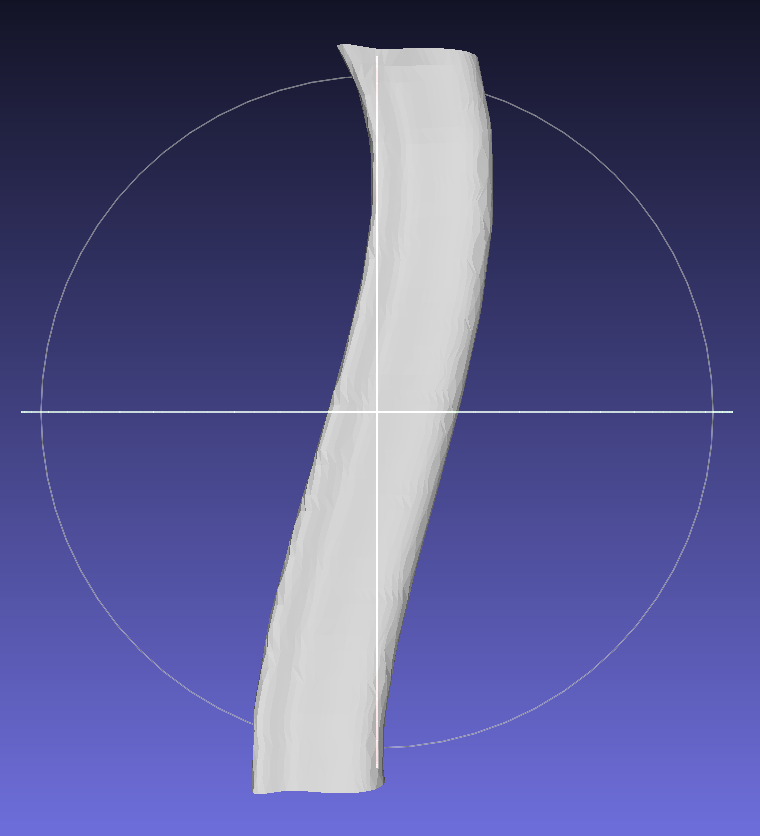
\includegraphics[width=.48\linewidth]{reconstructions/dtw-simple-50}}%
       \hfill
       \subcaptionbox{DTW 10 planes}
       {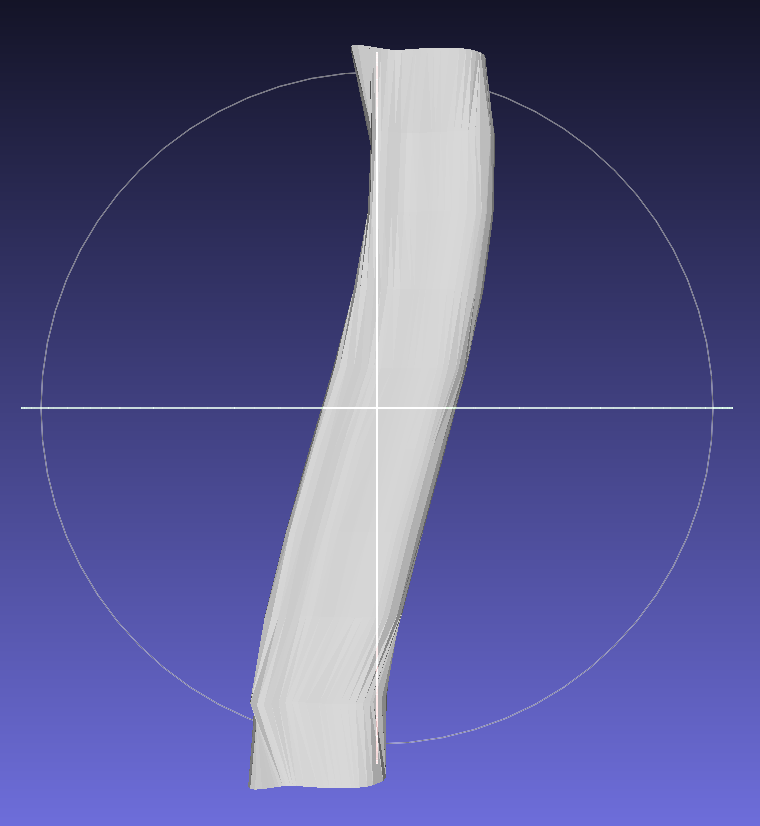
\includegraphics[width=.48\linewidth]{reconstructions/dtw-simple-10}}
       \hfill
       \subcaptionbox{CSPA 50 planes}
       {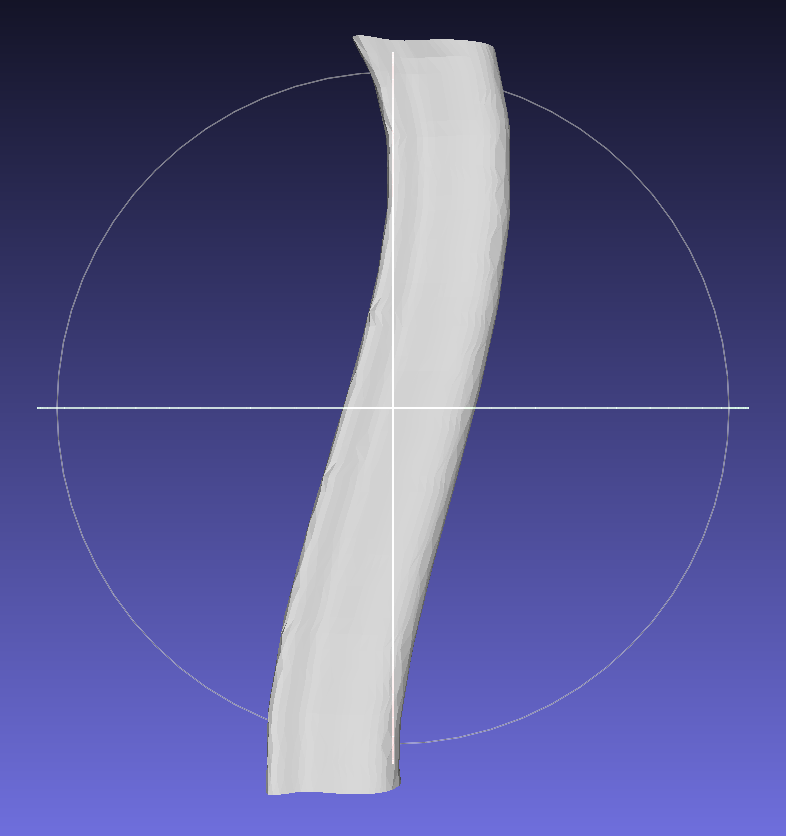
\includegraphics[width=.48\linewidth]{reconstructions/cspa50-simple-50}}%
       \hfill
       \subcaptionbox{CSPA 10 planes}
       {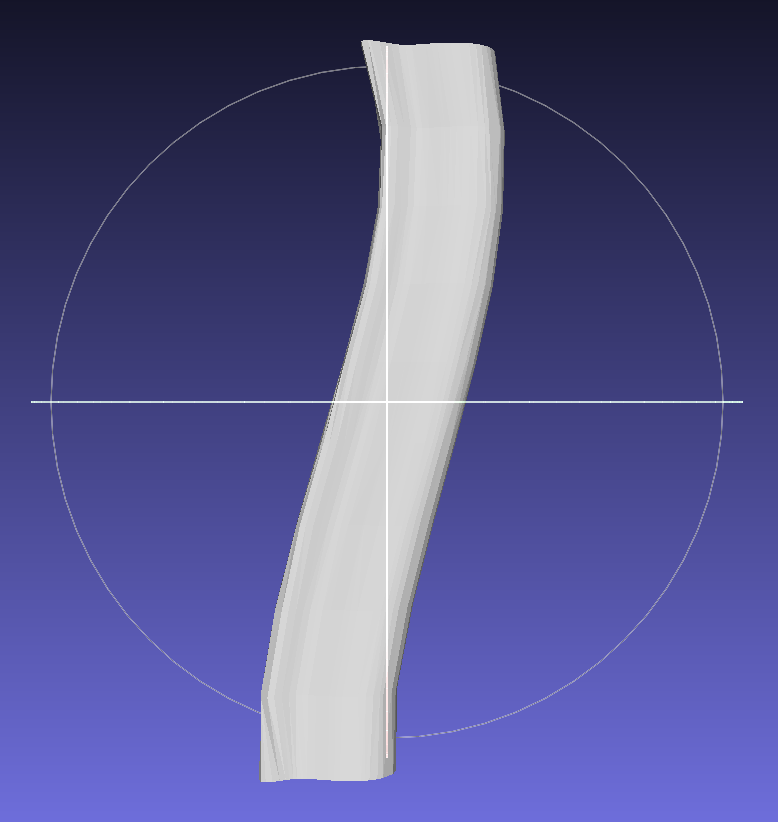
\includegraphics[width=.48\linewidth]{reconstructions/cspa50-simple-10}}
     \end{minipage}%
        \caption{Reconstructions of simple model}
        \label{fig:simple_reconstructions}
\end{figure}

Both reconstruction methods handle this simple case well, with both 50 and 10 plane samples. In the 10 plane reconstruction, they both have visible jagged parts at the bottom, although CSPA seems to be better in this area. We now look at Hausdorff distance to confirm this.

\begin{table}[h!]
\begin{tabular}{ | c | c | c | c | c | c | }
\hline
& \multicolumn{5}{c|}{No. of Slices Sampled} \\
\cline{2-6}
Method & 10 & 20 & 30 & 40 & 50 \\
\hline
Contour Merging + DTW & 0.0368 & 0.0274 & 0.0174 & 0.0195 & 0.0145 \\
Contour Splitting + Point Angle (CSPA) & 0.0297 & 0.0240 & 0.0165 & 0.0190 & 0.0140 \\
\hline
\end{tabular}
\caption{Simple model, mean Hausdorff distance from original to reconstruction}
\label{table:simple_forward}
\end{table}

In Table \ref{table:simple_forward}, the anamoly at 40 samples (being higher than expected) is caused by the 40 plane samples not spanning the full original model. This affects both methods equivalently so has been left in for relative comparison.

\begin{table}[h!]
\begin{tabular}{ | c | c | c | c | c | c | }
\hline
& \multicolumn{5}{c|}{No. of Slices Sampled} \\
\cline{2-6}
Method & 10 & 20 & 30 & 40 & 50 \\
\hline
Contour Merging + DTW & 0.0186 & 0.00836 & 0.00479 & 0.00336 & 0.00275 \\
Contour Splitting + Point Angle (CSPA) & 0.0102 & 0.00401 & 0.00281 & 0.00236 & 0.00215 \\
\hline
\end{tabular}
\caption{Simple model, mean Hausdorff distance from reconstruction to original}
\label{table:simple_reverse}
\end{table}

\begin{figure}[h!]
\centering
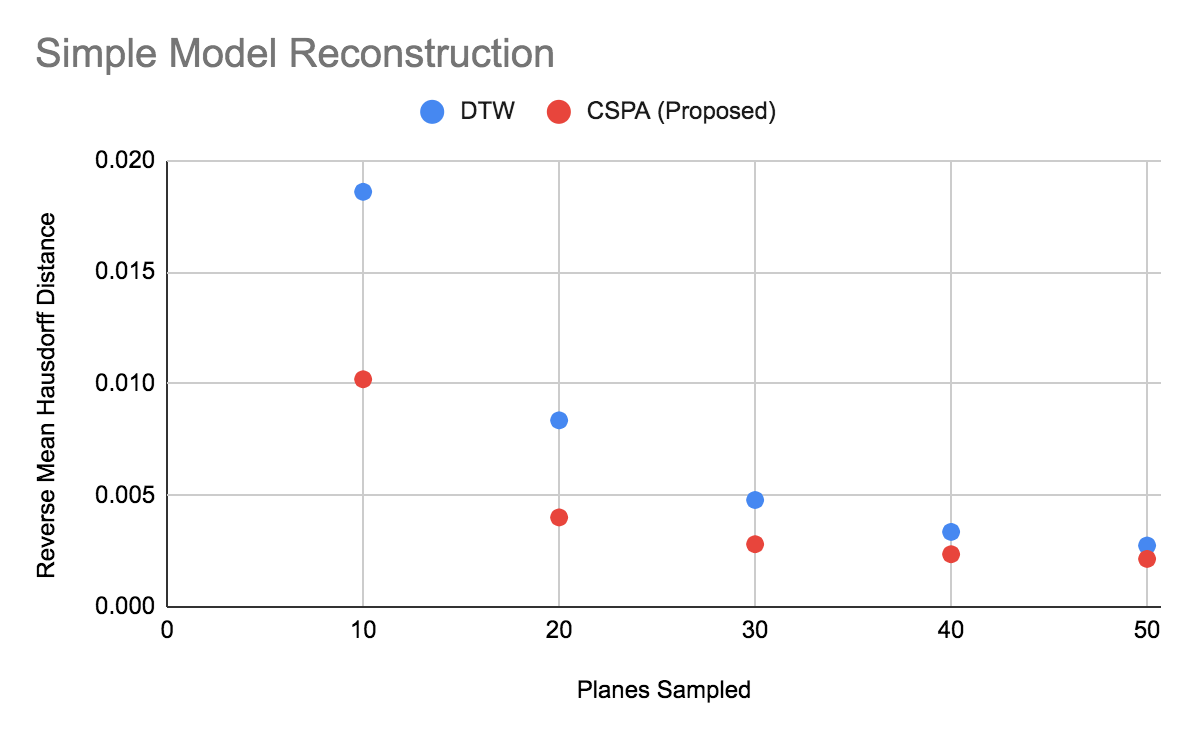
\includegraphics[width=0.9\textwidth]{graphs/simple-reverse}
\caption{Simple model, mean Hausdorff distance from reconstruction to original\label{fig:simple_reverse_graph}}
\end{figure}

As we can see from Table \ref{table:simple_reverse} and Figure \ref{fig:simple_reverse_graph}, our data agrees with the trend in Mackay's measurements, in that more slices sampled results in more accurate reconstructions. At high sample rates, the two methods have similar accuracies. However, as the sample rate lowers, CSPA has better measured accuracy than DTW. This is a trend which will continue for the remaining models.
\pagebreak

\subsubsection{Simple Branch Reconstruction}

A simple model containing a branch is reconstructed. Here there are cases where contour correspondence is invalid (for 20 and 50 plane samples), and 40 plane samples has an issue which will be explained later, so only 10 and 30 plane samples are shown first.

\begin{figure}[h!]
     \centering
     \begin{minipage}[b]{\reconstructionleft\linewidth}
       \subcaptionbox{Original}
       {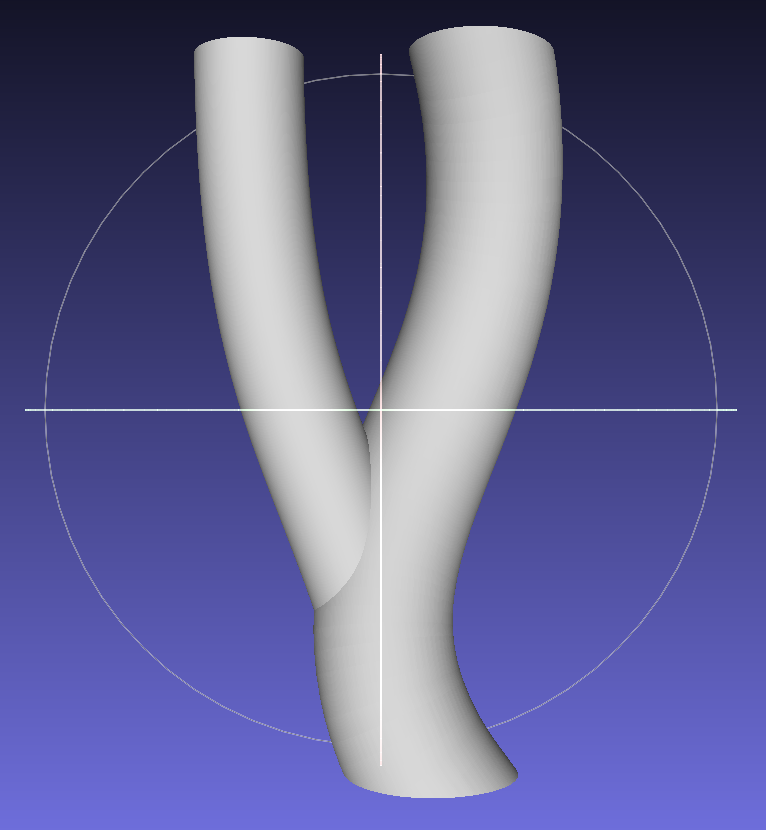
\includegraphics[width=\linewidth]{originals/simple-branch}}%
     \end{minipage}%
     \hfill
     \begin{minipage}[b]{\reconstructionright\linewidth}
       \subcaptionbox{DTW 30 planes}
       {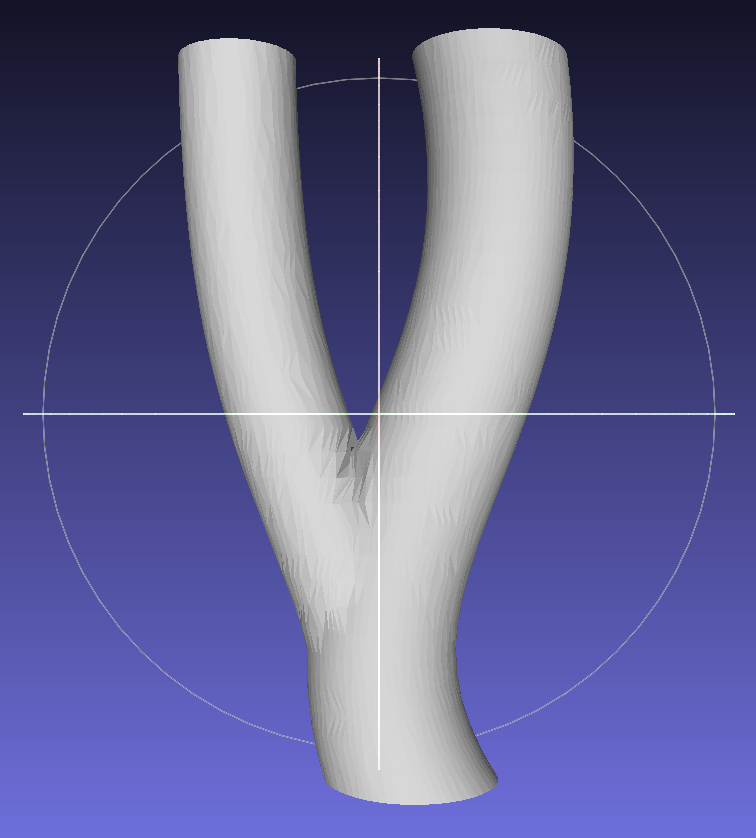
\includegraphics[width=0.48\linewidth]{reconstructions/dtw-simple-branch-30}}%
       \hfill
       \subcaptionbox{DTW 10 planes}
       {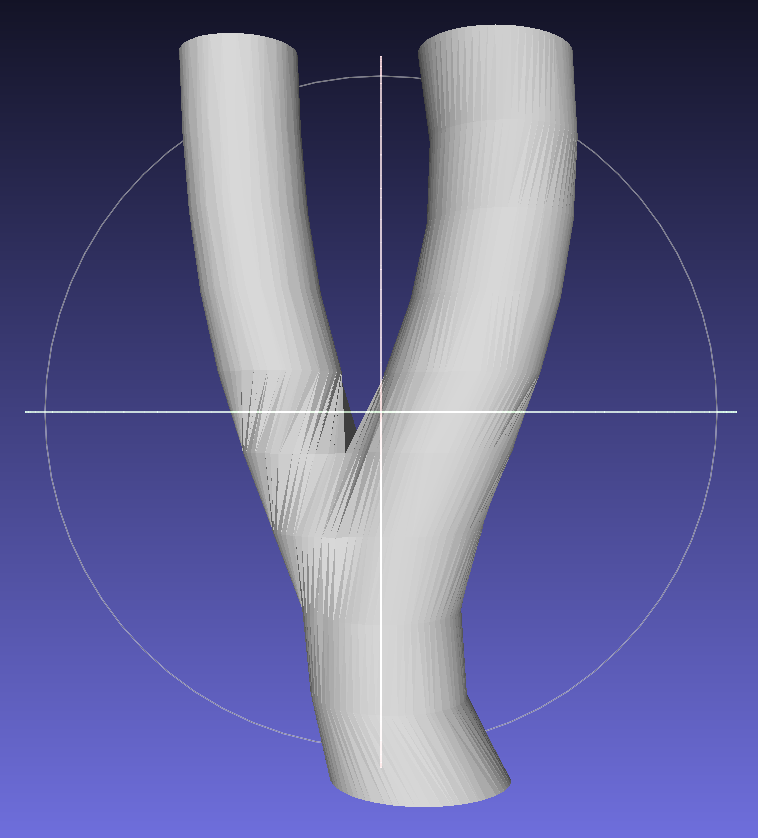
\includegraphics[width=.48\linewidth]{reconstructions/dtw-simple-branch-10}}
       \hfill
       \subcaptionbox{CSPA 30 planes}
       {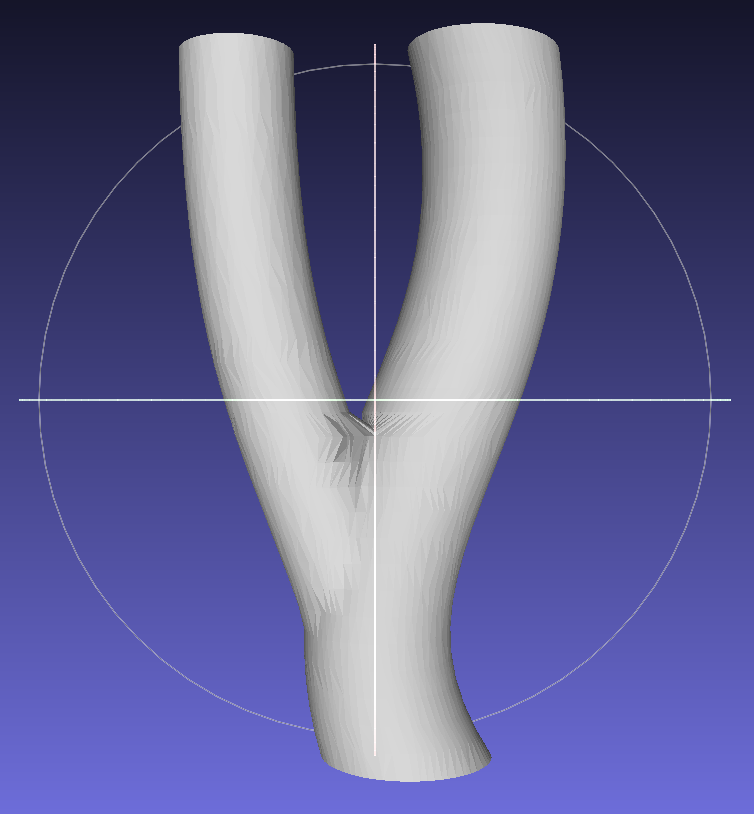
\includegraphics[width=.48\linewidth]{reconstructions/cspa50-simple-branch-30}}%
       \hfill
       \subcaptionbox{CSPA 10 planes}
       {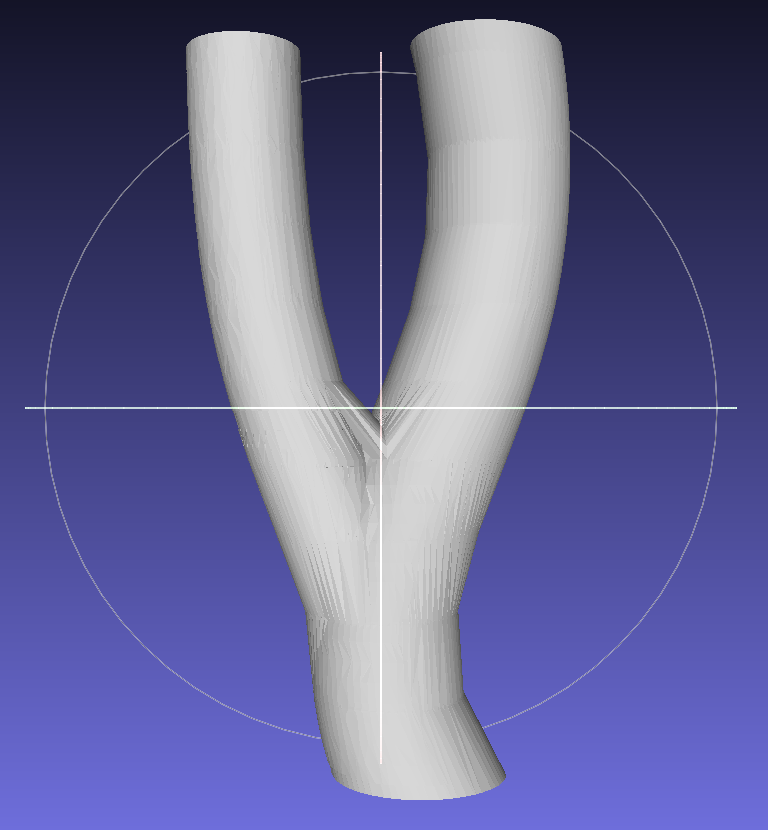
\includegraphics[width=.48\linewidth]{reconstructions/cspa50-simple-branch-10}}
     \end{minipage}%
        \caption{Reconstructions of simple branch model}
        \label{fig:simple_branch_reconstructions}
\end{figure}

At 30 plane samples we see decent reconstructions, with CSPA having a slightly less clean split. At 10 plane samples, DTW reconstructs one side of the branch well, but the other side is twisted, and the split is missing triangles. CSPA on the other hand has a clean reconstruction in terms of being closed and smooth on the branches, but there is an obvious protrusion where the split line has been slightly misplaced. 

These 10-plane figures highlight the behaviours of the two approaches. With merging + DTW, the constraints on DTW force the point correspondence to move along on both sides. When the correspondence arrives at one of the merging points on the two-contour, it can only connect to a few points on the single contour before being forced to jump across the merge. This results in the split on the single contour being placed not exactly halfway between the branches. In Figure \ref{fig:simple_branch_reconstructions}, this is visible as the front split being more left than it should. With CSPA, the split line is placed based on an estimation of the ratio of areas of the two contours, and the ratio of areas in the split contour. This gets the split line close to where it should be, but not exactly. In Figure \ref{fig:simple_branch_reconstructions}, we see it has estimated the split line to be further right than it should be. Perhaps a metric accounting for contour shape to find where the single contour starts to pinch would be more accurate, but also more sensitive to irregular contour shapes.

\begin{table}[h!]
\begin{tabular}{ | c | c | c | c | c | c | }
\hline
& \multicolumn{5}{c|}{No. of Slices Sampled} \\
\cline{2-6}
Method & 10 & 20 & 30 & 40 & 50 \\
\hline
Contour Merging + DTW & 0.0727 & - & 0.0641 & 0.0605 & - \\
Contour Splitting + Point Angle (CSPA) & 0.0685 & - & 0.0640 & 0.0607 & - \\
\hline
\end{tabular}
\caption{Simple branch model, mean Hausdorff distance from original to reconstruction}
\label{table:simple_branch_forward}
\end{table}
\FloatBarrier

\begin{table}[h!]
\begin{tabular}{ | c | c | c | c | c | c | }
\hline
& \multicolumn{5}{c|}{No. of Slices Sampled} \\
\cline{2-6}
Method & 10 & 20 & 30 & 40 & 50 \\
\hline
Contour Merging + DTW & 0.0195 & - & 0.0107 & 0.0538 & - \\
Contour Splitting + Point Angle (CSPA) & 0.0147 & - & 0.0115 & 0.0768 & - \\
\hline
\end{tabular}
\caption{Simple branch model, mean Hausdorff distance from reconstruction to original}
\label{table:simple_branch_reverse}
\end{table}
\FloatBarrier

For higher plane counts the two methods have almost equal accuracy, with CSPA actually being worse at 40 plane samples. At a plane count of 10, CSPA is more accurate. The 40 plane sample version has poor accuracy for both reconstructions. Inspecting the models (See Figure \ref{fig:simple_branch_40}), the issue appears to be with triangulation of the point correspondences, rather than a bad contour correspondence. This may be worth investigating, to see if this is an input case needing improvement or an implementation error.

\begin{figure}[h!]
     \centering
     \begin{subfigure}[b]{0.45\textwidth}
         \centering
         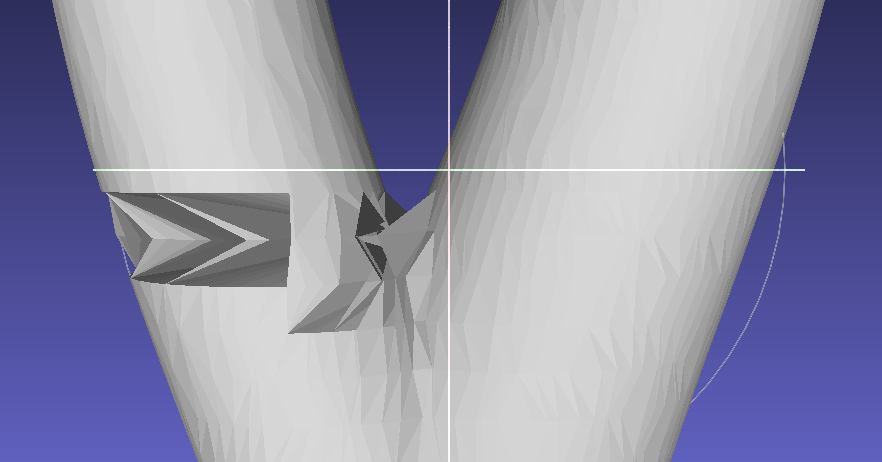
\includegraphics[width=\textwidth]{reconstructions/dtw-simple-branch-40}
         \caption{DTW}
         \label{fig:dtw_simple_branch_40}
     \end{subfigure}
     \hfill
     \begin{subfigure}[b]{0.45\textwidth}
         \centering
         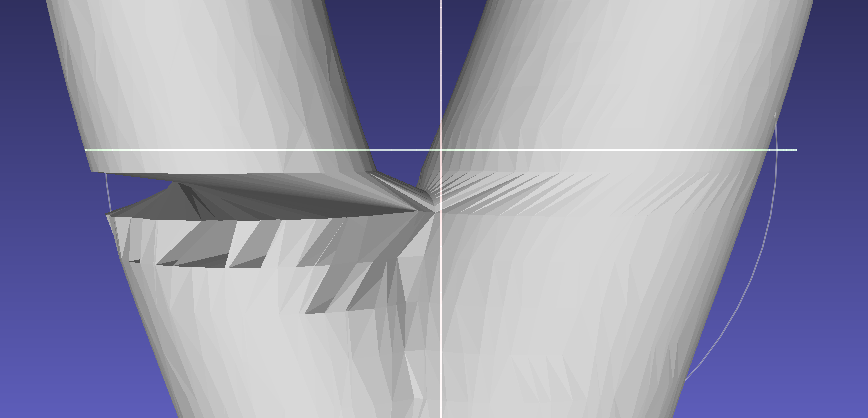
\includegraphics[width=\textwidth]{reconstructions/cspa50-simple-branch-40}
         \caption{CSPA}
         \label{fig:cspa50_simple_branch_40}
     \end{subfigure}
        \caption{Simple branch reconstruction error}
        \label{fig:simple_branch_40}
\end{figure}

I follow this up with a model containing only the branch section of the simple branch model. I compared the complete simple model reconstruction to this focussed original model, to specifically see Hausdorff distance at the branch section. Only the forward Hausdorff distance is valid here.

\begin{figure}[h!]
\centering
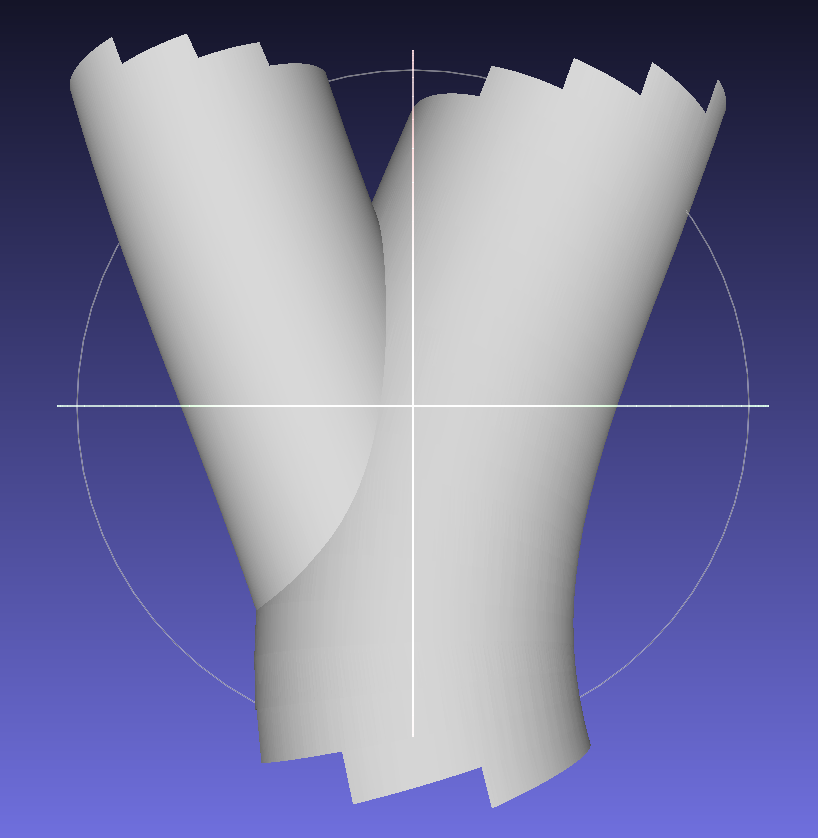
\includegraphics[width=0.3\textwidth]{originals/simple-branch-2-6}
\caption{Simple branch model focussed on the branch\label{fig:simple_branch_focussed}}
\end{figure}

\begin{table}[h!]
\begin{tabular}{ | c | c | c | c | c | c | }
\hline
& \multicolumn{5}{c|}{No. of Slices Sampled} \\
\cline{2-6}
Method & 10 & 20 & 30 & 40 & 50 \\
\hline
Contour Merging + DTW & 0.0315 & - & 0.00453 & 0.00440 & - \\
Contour Splitting + Point Angle (CSPA) & 0.0207 & - & 0.00469 & 0.00482 & - \\
\hline
\end{tabular}
\caption{Simple branch focussed model, mean Hausdorff distance from original to reconstruction}
\label{table:simple_branch_focussed_forward}
\end{table}

This effectively shows the same results as the complete version of the model. 
\pagebreak

\subsubsection{Multi Branch Reconstruction}

A model with multiple branches at different orientations is reconstructed.

\begin{figure}[h!]
     \centering
     \begin{minipage}[b]{\reconstructionleft\linewidth}
       \subcaptionbox{Original}
       {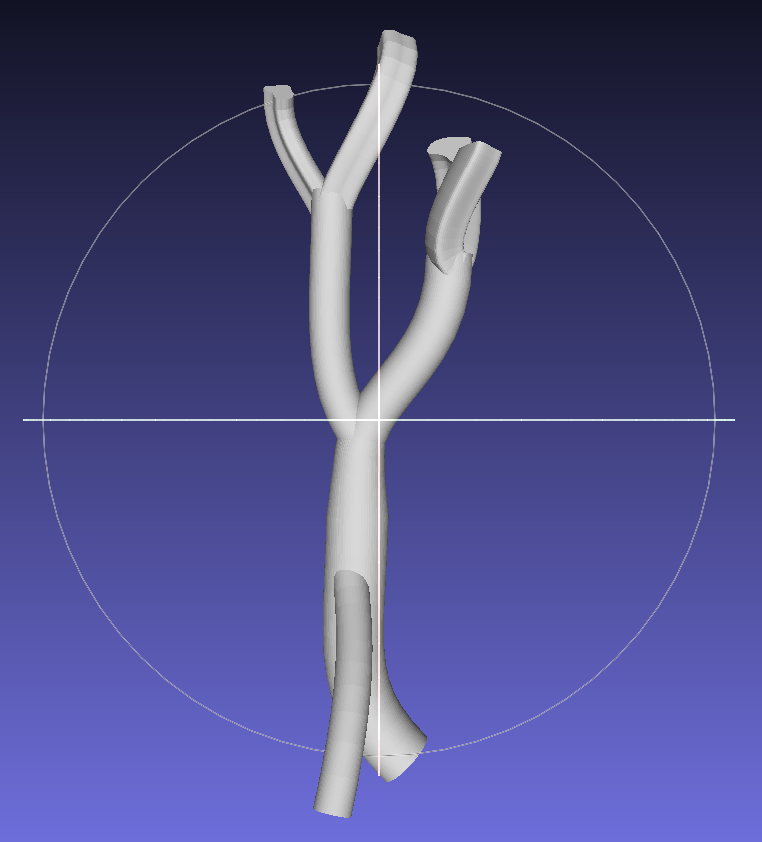
\includegraphics[width=\linewidth]{originals/multi-branch}}%
     \end{minipage}%
     \hfill
     \begin{minipage}[b]{\reconstructionright\linewidth}
       \subcaptionbox{DTW 50 planes}
       {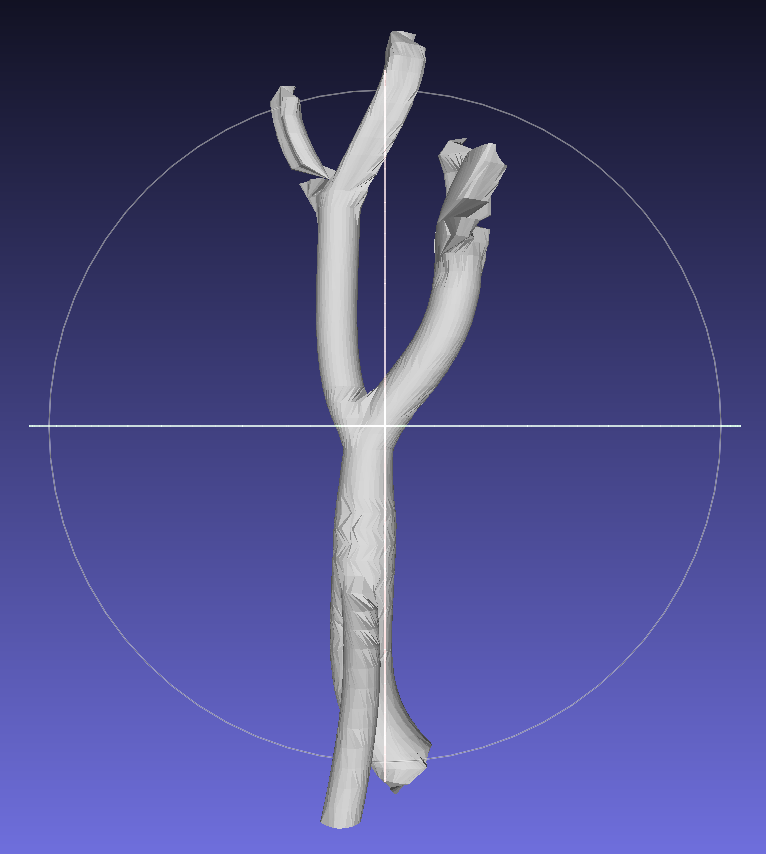
\includegraphics[width=.48\linewidth]{reconstructions/dtw-multi-branch-50}}%
       \hfill
       \subcaptionbox{DTW 10 planes}
       {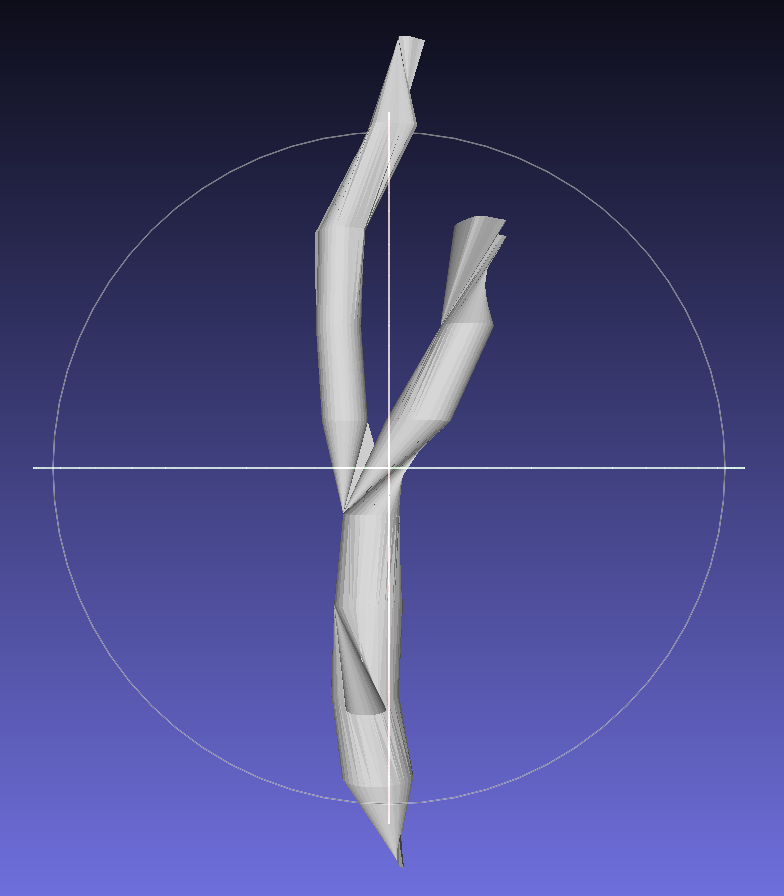
\includegraphics[width=.48\linewidth]{reconstructions/dtw-multi-branch-10}}
       \hfill
       \subcaptionbox{CSPA 50 planes}
       {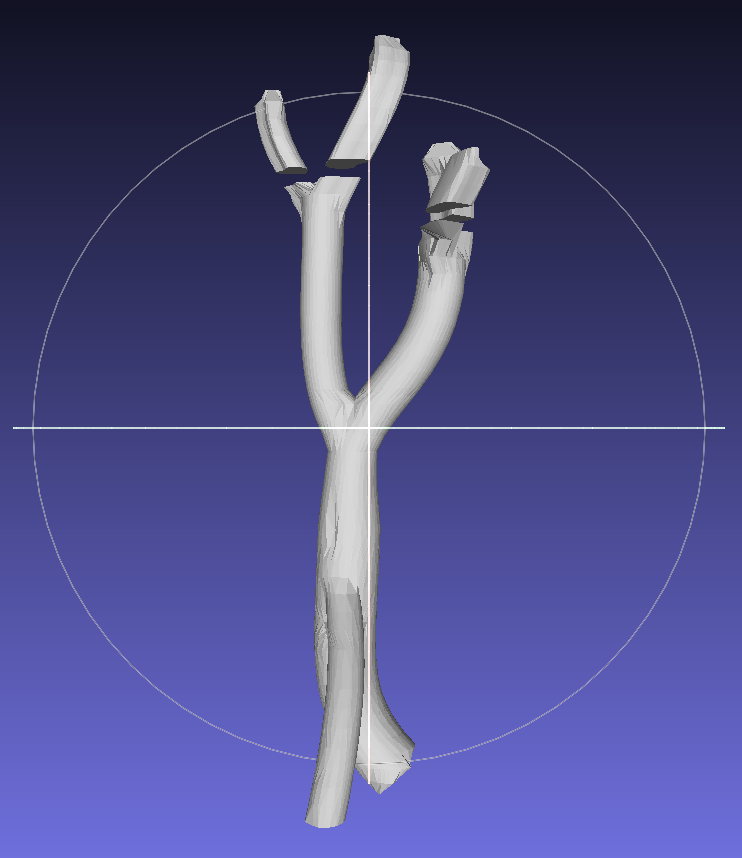
\includegraphics[width=.48\linewidth]{reconstructions/cspa50-multi-branch-50}}%
       \hfill
       \subcaptionbox{CSPA 10 planes}
       {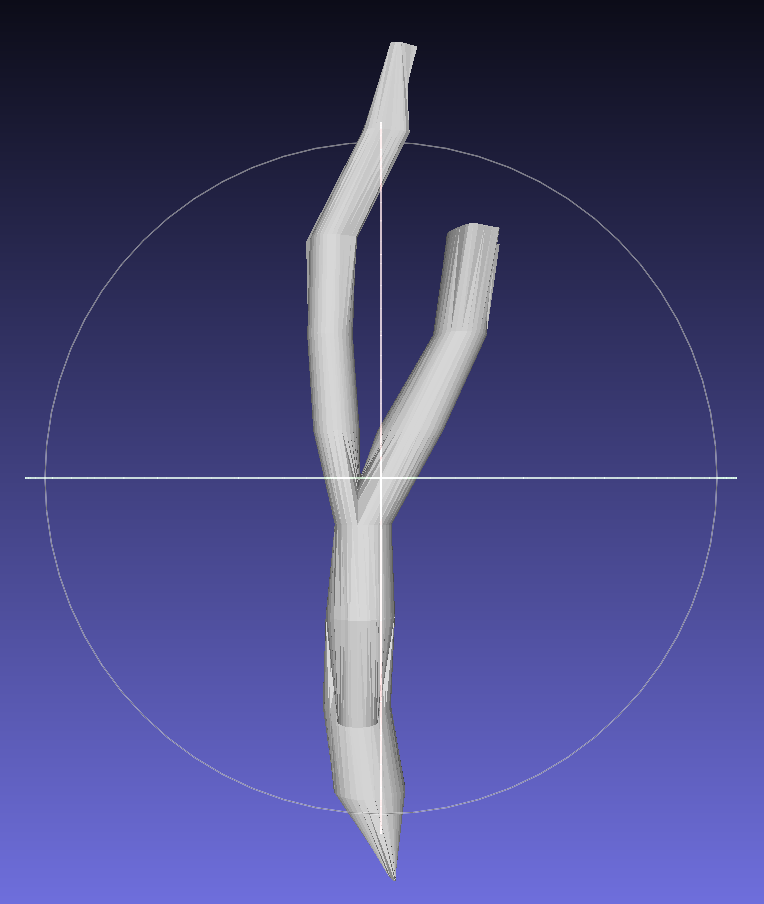
\includegraphics[width=.48\linewidth]{reconstructions/cspa50-multi-branch-10}}
     \end{minipage}%
        \caption{Reconstructions of multi branch model}
        \label{fig:multi_branch_reconstructions}
\end{figure}

In the branches with correct contour correspondence (the middle and lower branches), we can compare the point correspondence. In the 50-plane reconstructions, we see similar quality in the middle branch from both methods. However in the lower branch, CSPA produces a smoother point correspondence. In the 10-plane reconstructions, DTW has bad artefacts in both branches, such as twisting, and too many points being matched to a single point. CSPA solves these problems, giving better branch reconstructions.

The 50-plane reconstructions show invalid contour correspondence in the top branches. In the 10-plane versions, entire branch halves are missing from the contour correspondence. These issues affect most of the multi-branch reconstructions. For the latter reason we will consider only the reverse Hausdorff distance, from reconstruction to original. Note that this favours CSPA more as its implementation omits some sections with invalid contour correspondence, and so that section is not sampled from. For this reason we will revisit a version of this model focussing only on the lower two branches.

\begin{table}[h!]
\begin{tabular}{ | c | c | c | c | c | c | }
\hline
& \multicolumn{5}{c|}{No. of Slices Sampled} \\
\cline{2-6}
Method & 10 & 20 & 30 & 40 & 50 \\
\hline
Contour Merging + DTW & 0.0964 & 0.0469 & 0.0320 & 0.0400 & 0.0236 \\
Contour Splitting + Point Angle (CSPA) & 0.0773 & 0.0371 & 0.0157 & 0.0350 & 0.0135 \\
\hline
\end{tabular}
\caption{Multi branch model, mean Hausdorff distance from reconstruction to original}
\label{table:multi_branch_reverse}
\end{table}
\FloatBarrier

\begin{figure}[h!]
\centering
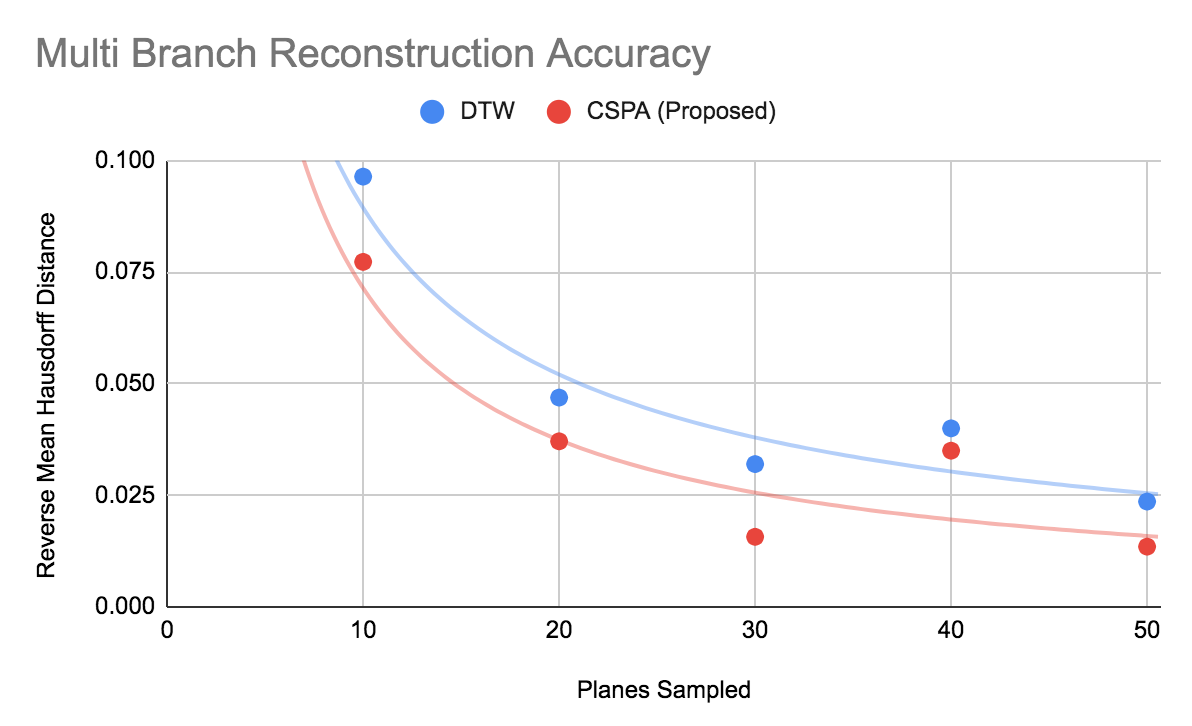
\includegraphics[width=0.9\textwidth]{graphs/multi-branch-reverse}
\caption{Multi branch reconstruction, mean Hausdorff distance from reconstruction to original\label{fig:multi_branch_reverse_graph}}
\end{figure}

The reverse mean Hausdorff distance indicates CSPA gives more accurate reconstructions of the multi branch model than DTW at all plane sample counts. To confirm this is not down to the omissions caused by the CSPA implementation, we use the focussed multi-branch model. As with the simple branch focussed, only forward Hausdorff distance is valid here.

\begin{figure}[h!]
\centering
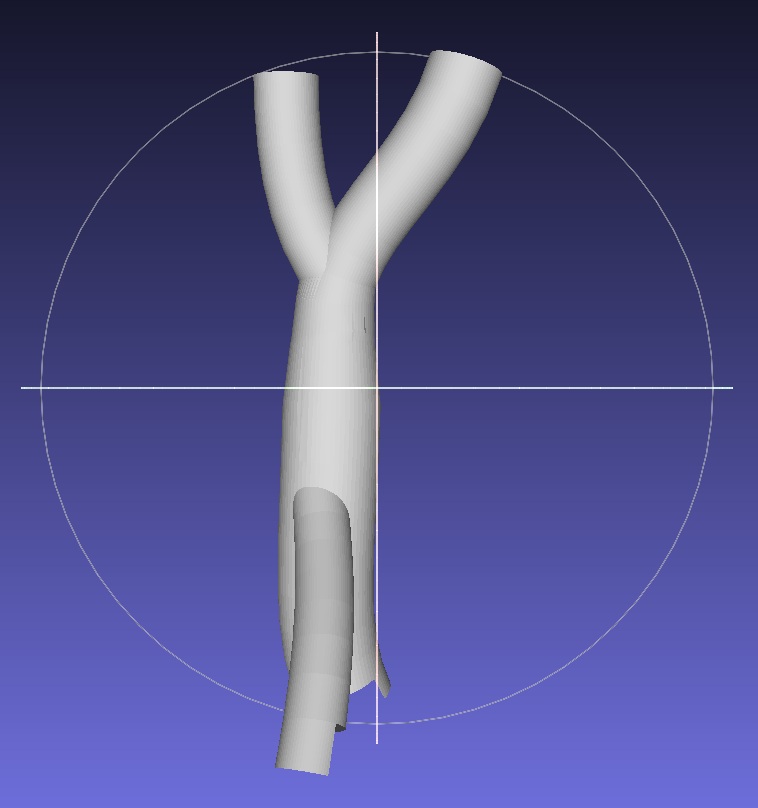
\includegraphics[width=0.3\textwidth]{originals/multi-branch-2-7}
\caption{Multi branch model focussed on lower two branches\label{fig:multi_branch_focussed}}
\end{figure}

\begin{table}[h!]
\begin{tabular}{ | c | c | c | c | c | c | }
\hline
& \multicolumn{5}{c|}{No. of Slices Sampled} \\
\cline{2-6}
Method & 10 & 20 & 30 & 40 & 50 \\
\hline
Contour Merging + DTW & 0.149 & 0.0238 & 0.0134 & 0.0109 & 0.00674 \\
Contour Splitting + Point Angle (CSPA) & 0.143 & 0.0175 & 0.00934 & 0.0108 & 0.00497 \\
\hline
\end{tabular}
\caption{Multi branch focussed model, mean Hausdorff distance from original to reconstruction}
\label{table:multi_branch_focussed_forward}
\end{table}
\FloatBarrier

These Hausdorff distances show that CSPA either equates with or improves in accuracy compared to DTW in the lower branching sections.
\pagebreak

\subsubsection{Bend Reconstruction}

In this section a bended tube is reconstructed. This tube is oriented so that when scanned, it appears as two contours coming down to one, similar to a branch.

\begin{figure}[h!]
     \centering
     \begin{minipage}[b]{\reconstructionleft\linewidth}
       \subcaptionbox{Original}
       {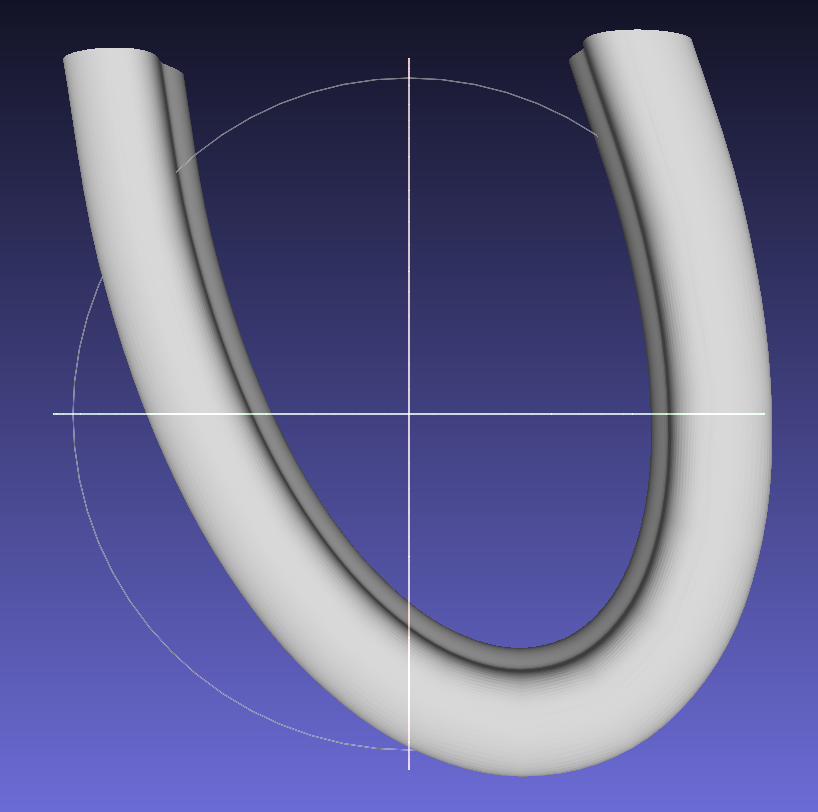
\includegraphics[width=\linewidth]{originals/bend}}%
     \end{minipage}%
     \hfill
     \begin{minipage}[b]{\reconstructionright\linewidth}
       \subcaptionbox{DTW 50 planes}
       {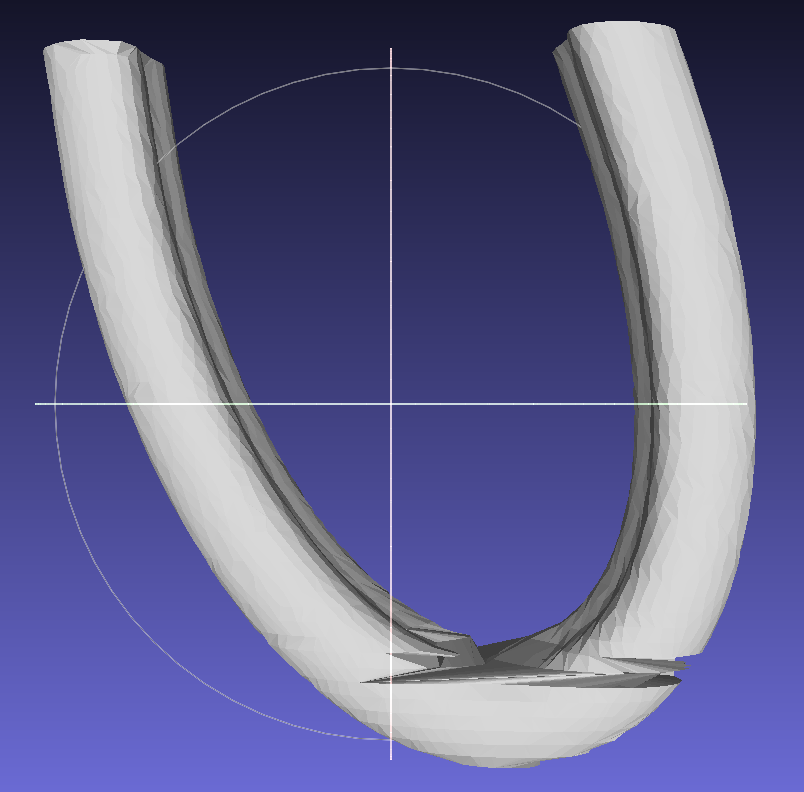
\includegraphics[width=.48\linewidth]{reconstructions/dtw-bend-50}}%
       \hfill
       \subcaptionbox{DTW 10 planes}
       {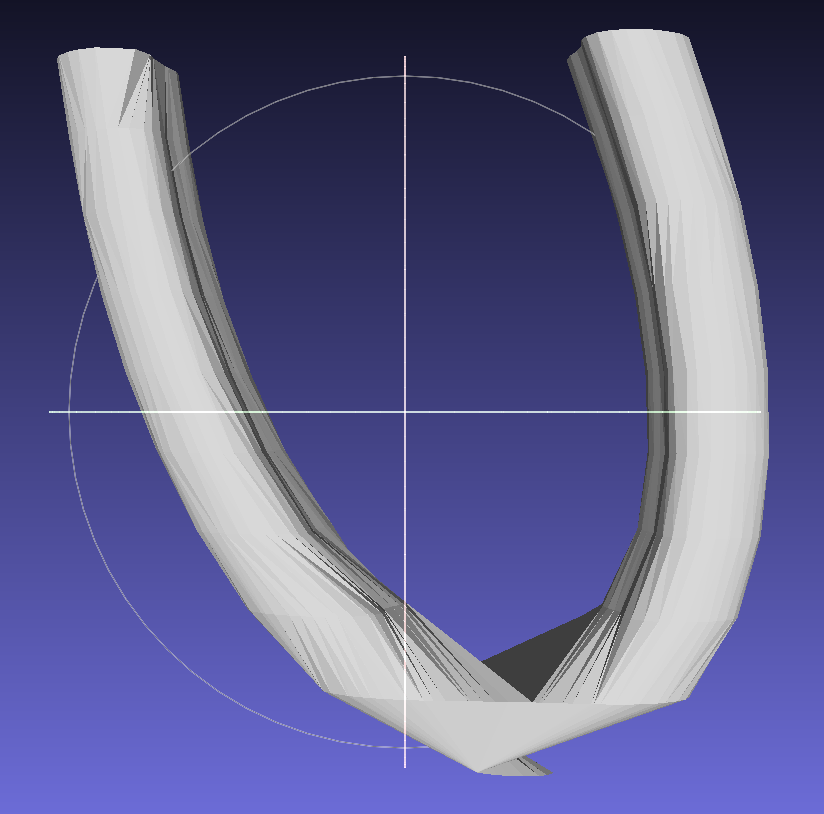
\includegraphics[width=.48\linewidth]{reconstructions/dtw-bend-10}}
       \hfill
       \subcaptionbox{CSPA 50 planes}
       {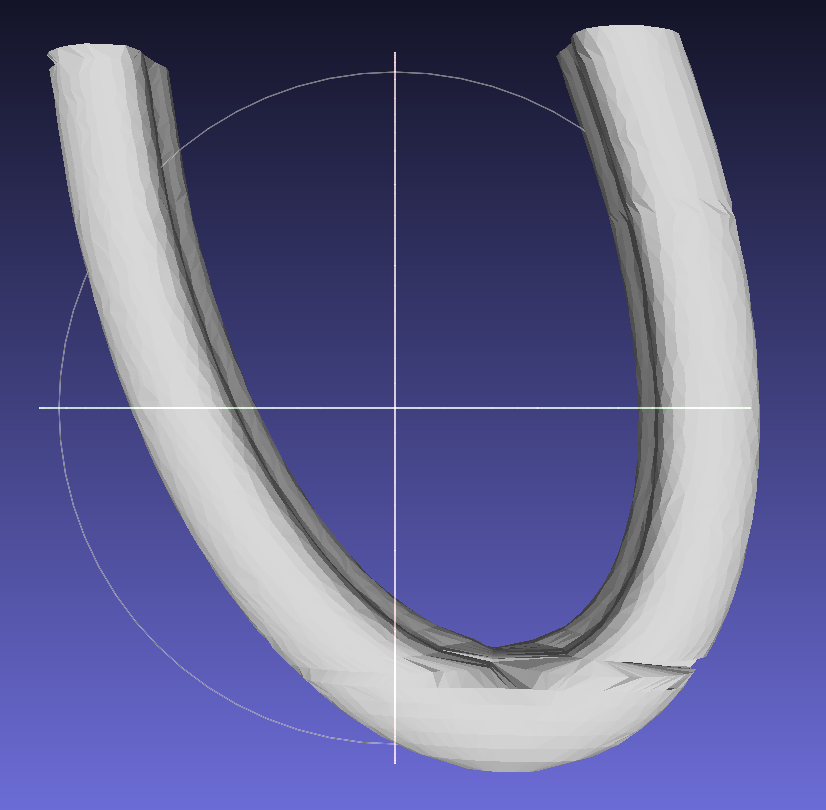
\includegraphics[width=.48\linewidth]{reconstructions/cspa50-bend-50}}%
       \hfill
       \subcaptionbox{CSPA 10 planes}
       {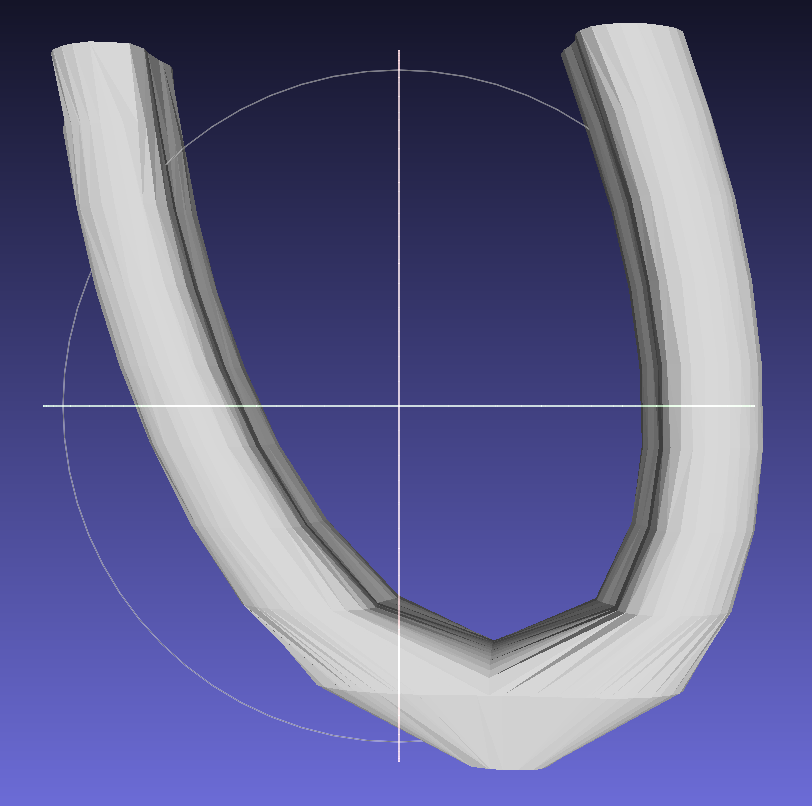
\includegraphics[width=.48\linewidth]{reconstructions/cspa50-bend-10}}
     \end{minipage}%
        \caption{Reconstructions of bend model}
        \label{fig:bend_reconstructions}
\end{figure}

For any plane count on the bend model, CSPA appears to have a cleaner reconstruction than DTW.

\begin{table}[h!]
\begin{tabular}{ | c | c | c | c | c | c | }
\hline
& \multicolumn{5}{c|}{No. of Slices Sampled} \\
\cline{2-6}
Method & 10 & 20 & 30 & 40 & 50 \\
\hline
Contour Merging + DTW & 0.0764 & 0.0363 & 0.0321 & 0.0314 & 0.0266 \\
Contour Splitting + Point Angle (CSPA) & 0.0647 & 0.0325 & 0.0281 & 0.0296 & 0.0256 \\
\hline
\end{tabular}
\caption{Bend model, mean Hausdorff distance from original to reconstruction}
\label{table:bend_forward}
\end{table}

\begin{table}[h!]
\begin{tabular}{ | c | c | c | c | c | c | }
\hline
& \multicolumn{5}{c|}{No. of Slices Sampled} \\
\cline{2-6}
Method & 10 & 20 & 30 & 40 & 50 \\
\hline
Contour Merging + DTW & 0.0618 & 0.0313 & 0.0158 & 0.101 & 0.0752 \\
Contour Splitting + Point Angle (CSPA) & 0.0535 & 0.0173 & 0.0127 & 0.0650 & 0.0491 \\
\hline
\end{tabular}
\caption{Bend model, mean Hausdorff distance from reconstruction to original}
\label{table:bend_reverse}
\end{table}

For every plane count, CSPA reconstructions have a lower mean Hausdorrf distance than DTW, both in forward and reverse directions. Interestingly, the reverse Hausdorff distance is best for both at 30 plane samples, with worse accuracy as plane samples increase. I suspect this is because as the plane count increases, sampled contours get closer and closer to the part of the bend which is tangent to the planes. These contours are shaped more strangely, and both methods have worse accuracy reconstructing these. In the case of bends, lower plane count may be an advantage, provided the bend is not missed by any planes.

\begin{figure}[h!]
\centering
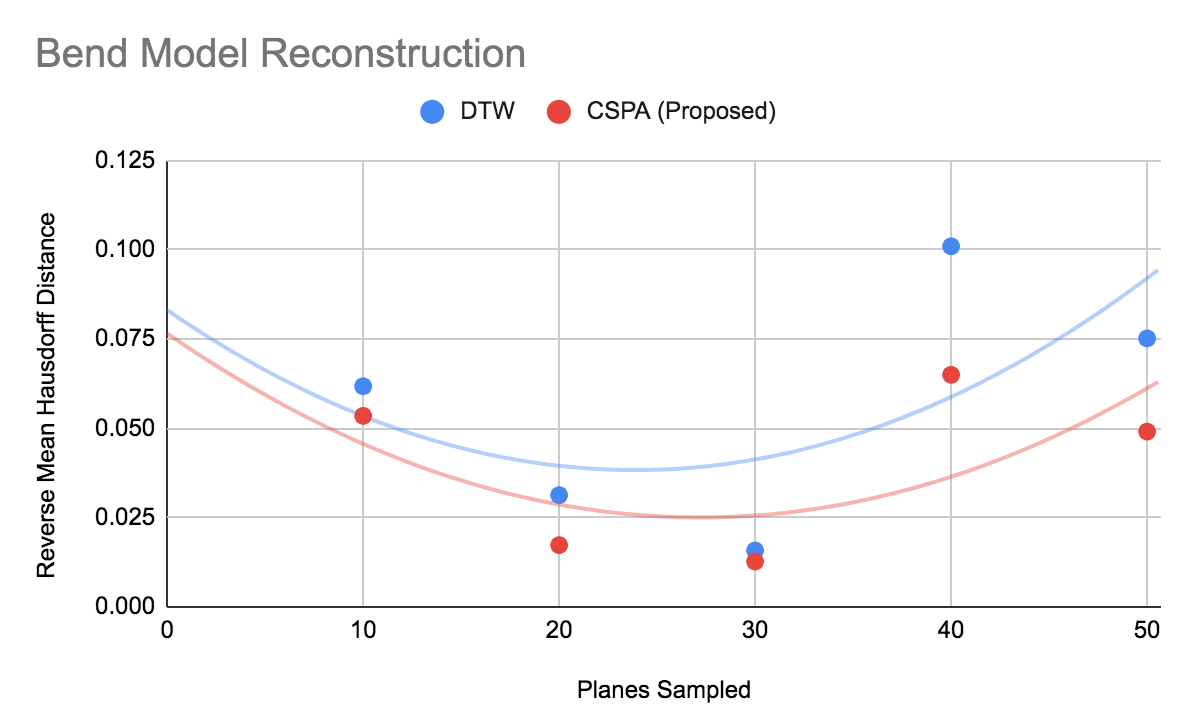
\includegraphics[width=0.9\textwidth]{graphs/bend-reverse}
\caption{Bend model, mean Hausdorff distance from reconstruction to original\label{fig:bend_reverse_graph}}
\end{figure}

\subsection{Angle Weight Comparison}

The point angle metric is a weighted sum of angle and progression for each point. The weighting given to both may influence how accurate CSPA reconstructions are. We will test this with the simple model and the multi-branch focussed model.

\begin{table}[h!]
\begin{tabular}{ | c | c | c | c | c | c | }
\hline
& \multicolumn{5}{c|}{Angle Weight} \\
\cline{2-6}
No. of Slices Sampled & 0\% & 25\% & 50\% & 75\% & 100\% \\
\hline
10 & 0.0107 & 0.0102 & 0.0102 & 0.0103 & 0.00998 \\
20 & 0.00457 & 0.00431 & 0.00401 & 0.00387 & 0.00380 \\
30 & 0.00329 & 0.00304 & 0.00281 & 0.00268 & 0.00264 \\
40 & 0.00296 & 0.00253 & 0.00236 & 0.00216 & 0.00216 \\
50 & 0.00277 & 0.00234 & 0.00215 & 0.00206 & 0.00204 \\
\hline
\end{tabular}
\caption{Angle weight comparison on simple model, mean Hausdorff distance from reconstruction to original}
\label{table:ang_weight_simple_reverse_transpose}
\end{table}

\begin{figure}[h!]
\centering
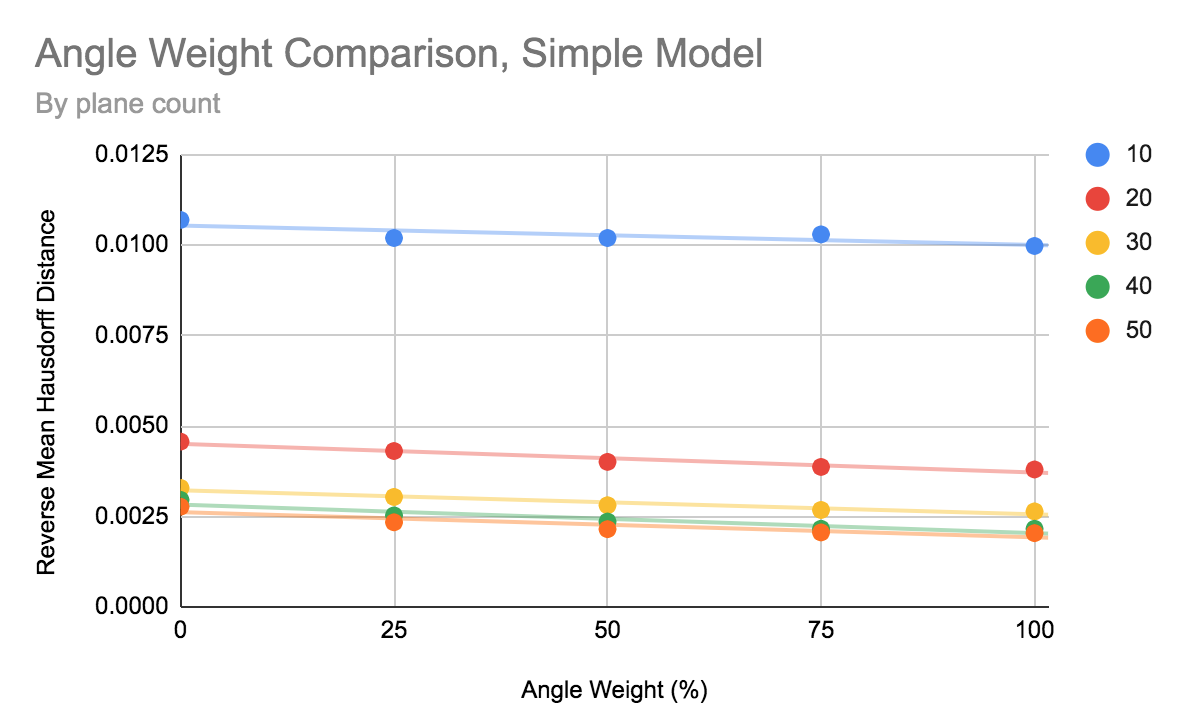
\includegraphics[width=0.9\textwidth]{graphs/ang_weight_simple_reverse}
\caption{Comparison of accuracy for various angle weights\label{fig:ang_weight_simple_reverse}}
\end{figure}
\FloatBarrier

For the simple model (See Table \ref{table:ang_weight_simple_reverse_transpose}) we can see that for every plane count, higher angle weight produces more accurate reconstructions. There seems to be diminishing returns on increasing angle weight, so using an angle weight of about 75\% could be a good way to keep some progression weighting, in order to handle more oddly shaped contours. At low plane counts such as 10, the effect of changing angle weight is lessened. These trends are just for a simple model synthetically produced, and so may not apply to real data. Robust behaviour across varying structures is probably more important than optimising accuracy for simpler cases, and the difference seen here is minimal. We now investigate the multi-branch focussed model.

\begin{table}[h!]
\begin{tabular}{ | c | c | c | c | c | c | }
\hline
& \multicolumn{5}{c|}{Angle Weight} \\
\cline{2-6}
No. of Slices Sampled & 0\% & 25\% & 50\% & 75\% & 100\% \\
\hline
10 & 0.146 & 0.145 & 0.143 & 0.143 & 0.142 \\
20 & 0.0203 & 0.0186 & 0.0175 & 0.0169 & 0.0166 \\
30 & 0.0124 & 0.0107 & 0.00934 & 0.00849 & 0.00803 \\
40 & 0.0144 & 0.0127 & 0.0109 & 0.0100 & 0.00973 \\
50 & 0.00689 & 0.00574 & 0.00497 & 0.00448 & 0.00437 \\
\hline
\end{tabular}
\caption{Angle weight comparison on multi branch focussed model, mean Hausdorff distance from original to reconstruction}
\label{table:ang_weight_multi_branch_focussed_forward_transpose}
\end{table}

For the multi-branch model, we see similar trends to the simple model. It appears the angle metric can handle the synthetic branching cases well enough to be better than the progression metric. Again, for more complicated real contours this may not be the case.
\pagebreak

\subsection{Real Lung Scan Reconstruction}

HRCT stacks are supplied by Dr. Anthony Butler, and cleared for research by the Health and Disability Ethics Committee, Ministry of Health (No. URB/10/EXP/002) \cite{health2010annual}.

Due to technical difficulties with the implementations, only some parts of the lung were reconstructed, which unfortunately did not include any branching structures. However we can verify that CSPA gets the simpler parts correct, by taking a look at the trachea.

\begin{figure}[h!]
     \centering
     \begin{subfigure}[b]{0.45\textwidth}
         \centering
         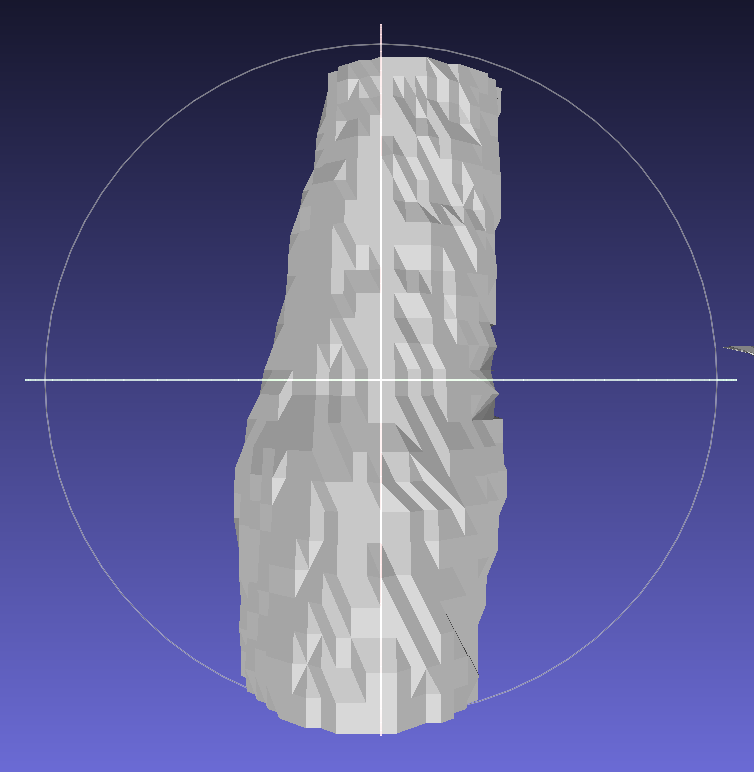
\includegraphics[width=\textwidth]{reconstructions/dtw-real}
         \caption{DTW}
         \label{fig:dtw_real}
     \end{subfigure}
     \hfill
     \begin{subfigure}[b]{0.45\textwidth}
         \centering
         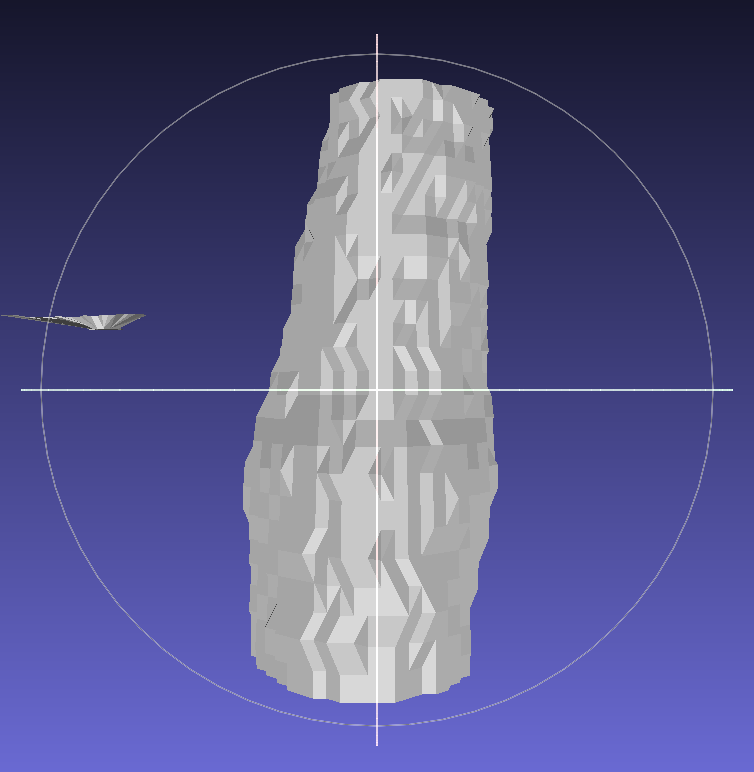
\includegraphics[width=\textwidth]{reconstructions/cspa50-real}
         \caption{CSPA (Proposed)}
         \label{fig:cspa50_real}
     \end{subfigure}
        \caption{Real trachea reconstruction, front side}
        \label{fig:real_reconstructions}
\end{figure}

In the scan data, the image resolution is similar to the plane thickness, and so we can see the individual triangles. Both methods have sufficient accuracy on the front side (Figure \ref{fig:real_reconstructions}) of the trachea.

\begin{figure}[h!]
     \centering
     \begin{subfigure}[b]{0.45\textwidth}
         \centering
         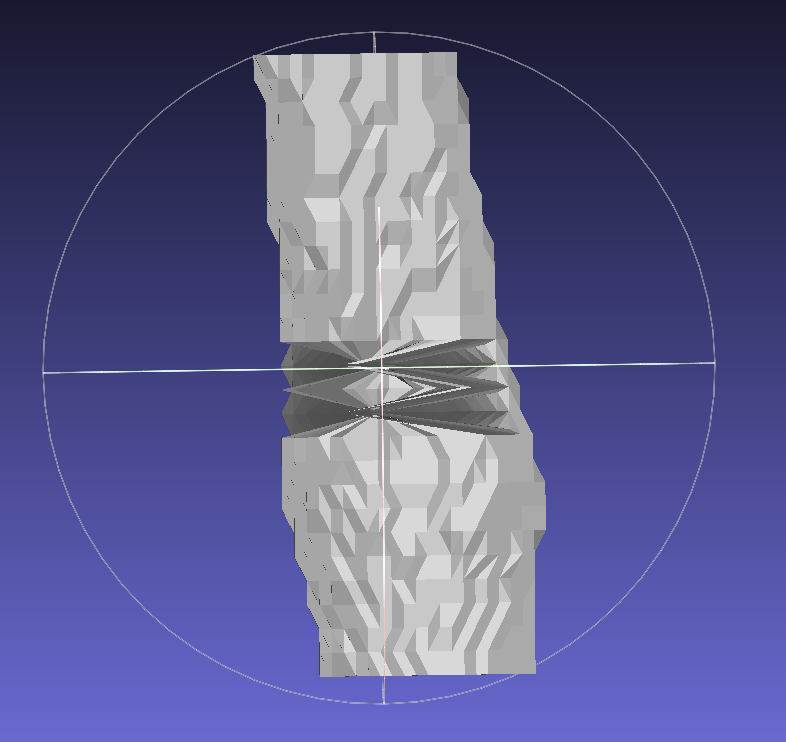
\includegraphics[width=\textwidth]{reconstructions/dtw-real-back}
         \caption{DTW}
         \label{fig:dtw_real_back}
     \end{subfigure}
     \hfill
     \begin{subfigure}[b]{0.45\textwidth}
         \centering
         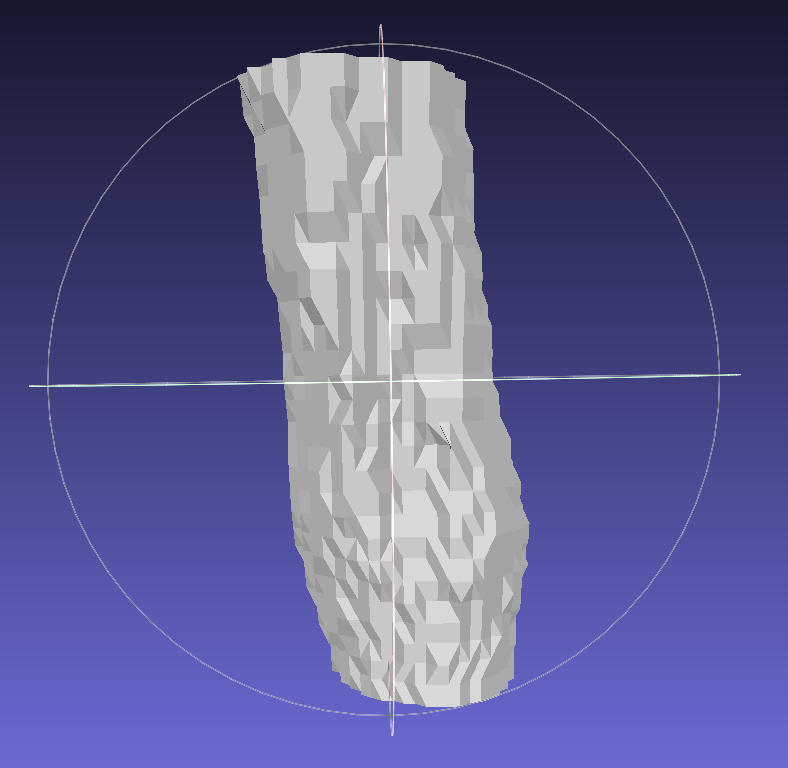
\includegraphics[width=\textwidth]{reconstructions/cspa50-real-back}
         \caption{CSPA (Proposed)}
         \label{fig:cspa50_real_back}
     \end{subfigure}
        \caption{Real trachea reconstruction, rear side}
        \label{fig:real_reconstructions_back}
\end{figure}

On the rear side (Figure \ref{fig:real_reconstructions_back}) we see DTW fail at a section with less circular contours (there is an indent which CSPA accurately reconstructs). This is a good indication that point angle may be superior to DTW in some instances. Further testing on more real data would be needed to establish whether this is consistent.
\pagebreak

\subsection{Performance}

We take a brief look at performance, to validate that even a naive implementation of contour splitting and point angle correspondence is not unreasonably inefficient.

PC specs:
\begin{itemize}
\item OS: macOS 10.13.4
\item CPU: 2.4 GHz dual core I5-4258U
\item RAM: 8GB DDR3
\item Disk: SSD
\item C++ compiled with debug flag
\end{itemize}

\begin{table}[h!]
\begin{tabular}{ | c | c | c | c | c | c | }
\hline
& \multicolumn{5}{c|}{No. of Slices Sampled} \\
\cline{2-6}
Method & 10 & 20 & 30 & 40 & 50 \\
\hline
Contour Merging + DTW & 35 & 54 & 92 & 106 & 147 \\
Contour Splitting + Point Angle (CSPA) & 36 & 45 & 70 & 79 & 98 \\
\hline
\end{tabular}
\caption{Time for one reconstruction of the simple model (ms)}
\label{table:performance_simple}
\end{table}

\begin{figure}[h!]
\centering
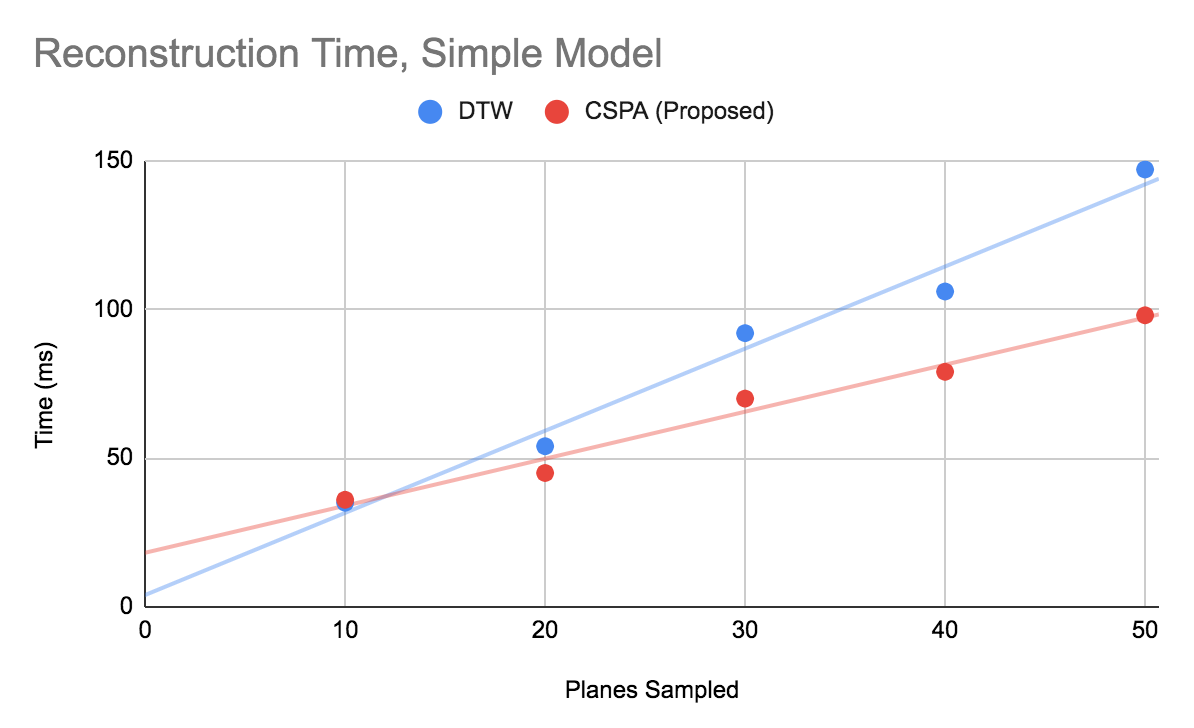
\includegraphics[width=0.9\textwidth]{graphs/performance-simple}
\caption{Performance of reconstruction methods on simple model\label{fig:performance_simple}}
\end{figure}
\FloatBarrier

CSPA performs at least as well as DTW, and even performs better as plane count goes up.

Next we turn to reconstruction performance on the multi branch model. 10 plane samples gives the highest proportion of contour correspondences which are branch cases. 

\begin{table}[h!]
\begin{tabular}{ | c | c | c | c | c | c | }
\hline
& \multicolumn{5}{c|}{No. of Slices Sampled} \\
\cline{2-6}
Method & 10 & 20 & 30 & 40 & 50 \\
\hline
Contour Merging + DTW & 44 & 65 & 94 & 115 & 140 \\
Contour Splitting + Point Angle (CSPA) & 29 & 44 & 58 & 90 & 104 \\
\hline
\end{tabular}
\caption{Time for one reconstruction of the multi branch model (ms)}
\label{table:performance_multi_branch}
\end{table}

\begin{figure}[h!]
\centering
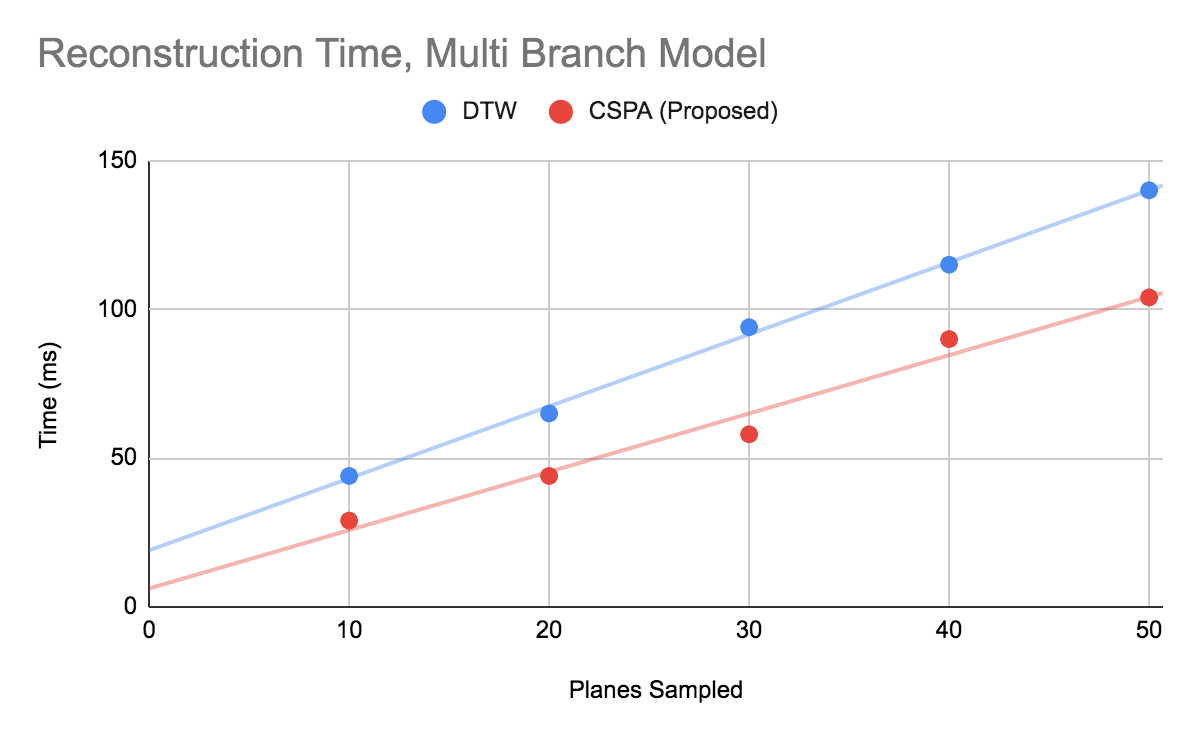
\includegraphics[width=0.9\textwidth]{graphs/performance-multi-branch}
\caption{Performance of reconstruction methods on multi branch model\label{fig:performance_multi_branch}}
\end{figure}
\FloatBarrier

In the branching cases, CSPA splits contours into separate point correspondences, and each correspondence has linear complexity. Mackay's implementation with merging creates larger contours for DTW to act on. Filling in the cost matrix gives DTW quadratic complexity, and so the slowdown for DTW relative to CSPA can probably be attributed to this. 

On the real dataset, DTW took an average of 88 seconds for a reconstruction, whilst CSPA took 83 seconds. Both implementations have some naive elements, but this is a good indicator that CSPA does not have any major flaws with regards to performance. It handles larger contours (on the order of hundreds of points) about as well as DTW.

\subsection{Analysis Summary}

CSPA gave more accurate reconstructions than DTW in branches and similar structures. As plane count lowered for a given object, CSPA's accuracy worsened at a rate slower than DTW's. This can be useful for reconstructing small objects. Also, there may be image stack data which has incomplete contour data (missing contours). In cases where contour correspondences traversing multiple slices are allowed, CSPA may handle the larger gap better.
\pagebreak

\section{Conclusion}

This paper proposes a new method for handling branching cases in point correspondence, and a new point correspondence algorithm. Contours are split in branching cases, and angle/progression metrics are used for point correspondence. The intent was to more deliberately choose key points in the point correspondence process (where splits occur, where correspondence starts from etc.). Synthetic models had contours sampled from them, to be reconstructed by the proposed method and the most comparable prior method by Mackay. The reconstructions were compared to the originals, with Hausdorff distance providing an accuracy metric. It was found that the proposed method on average handles branching cases better, especially at lower plane sample counts. Averaged across all models and plane sample counts, CSPA improved on DTW by an average of 15.2\%. Averaged across all models with 10 sample planes, there was an improvement of 17.5\%. The proposed method may provide an improvement for real applications with many branching cases and small objects, such as lung scans. The improvement in visual quality should help with understanding scanned structures, and the improvement in mesh quality and accuracy may help with further processing steps.

\subsection{Future Research}

Contour splitting is currently implemented to handle 1-to-2 cases. However the idea is simple enough to be generalised to 1-to-many. In addition, the ratio of areas can be explicitly calculated instead of approximated by number of points. This may cope with real contour shapes better. The split line curve can be modelled differently depending on factors such as how close the two contours are. For point correspondence, metrics other than point angle and progression can be considered.

Absent from the analysis was a reconstruction of a real branching structure. With a fixed contour correspondence, a comparison between DTW and CSPA (and other non-contour reconstruction methods) on real lung scans would be useful. An alternative would be to implement the synthetic lung model generation by Pluta et al. \cite{pluta2012new}. Sample planes could then be taken from this model and reconstructed, to allow for analysis on a more realistic structure than the models used in this paper.

Other ideas include:
\begin{itemize}
\item Contextual constraints on contour correspondence. For example, the lung bronchi should form a tree when corresponded.
\item Contour interpolation to reduce the difference between contours before point correspondence.
\item Triangulating branches as overlapping 1-to-1 cases, then merging the meshes produced.
\end{itemize}

\pagebreak
\bibliographystyle{IEEEtran}
\bibliography{references}

\end{document}
